\documentclass[10pt,a4paper,twoside]{article}

\usepackage[top=2.0cm, bottom=2.2cm, left=1.6cm, right=1.6cm]{geometry}
\usepackage{mathptmx}
\usepackage[scaled=0.92]{helvet}
\usepackage{amsmath,amssymb,amsfonts}
\usepackage{graphicx}
\graphicspath{{docs/figures/}}
\usepackage{booktabs}
\usepackage{xcolor}
\usepackage{fancyhdr}
\usepackage{caption}
\usepackage{cite}
\usepackage{microtype}
\usepackage{url}
\usepackage{multicol}
\usepackage{listings}
\usepackage[colorlinks=true, linkcolor=blue!70!black, citecolor=blue!70!black, urlcolor=blue!70!black]{hyperref}

% Lengths
\setlength{\columnsep}{0.65cm}
\setlength{\parindent}{11pt}

% Define colors
\definecolor{natureblue}{RGB}{0, 86, 179}
\definecolor{naturedark}{RGB}{11, 29, 58}
\definecolor{naturegray}{RGB}{100, 100, 100}
\definecolor{openorange}{RGB}{230, 100, 0}
\definecolor{alertred}{RGB}{180, 40, 40}
\definecolor{royalazure}{RGB}{0, 56, 175}

% Caption styling
\captionsetup{font=small, labelfont={bf,sf}, labelsep=period}

% Page headers and footers
\pagestyle{fancy}
\fancyhf{}
\renewcommand{\headrulewidth}{0.4pt}
\renewcommand{\footrulewidth}{0.4pt}
\fancyhead[LE]{\small\textsf{\textbf{npj Digital Medicine}}\quad\footnotesize\textsf{\textit{Preprint / Manuscript Under Review}}}
\fancyhead[RO]{\small\textsf{\textbf{npj Digital Medicine}}\quad\footnotesize\textsf{\textit{Preprint / Manuscript Under Review}}}
\fancyhead[LO]{\footnotesize\textsf{\textit{Symmetric evaluation of shallow quantum machine learning in healthcare}}}
\fancyhead[RE]{\footnotesize\textsf{\textit{Symmetric evaluation of shallow quantum machine learning in healthcare}}}
\fancyfoot[C]{\small\textsf{\thepage}}

\fancypagestyle{firstpage}{
  \fancyhf{}
  \renewcommand{\headrulewidth}{0pt}
  \renewcommand{\footrulewidth}{0.4pt}
  \fancyfoot[L]{\footnotesize\textsf{Prepared for submission to \textit{npj Digital Medicine}}}
  \fancyfoot[R]{\small\textsf{\thepage}}
}

% Section format
\makeatletter
\renewcommand{\section}{\@startsection{section}{1}{\z@}%
  {-2.2ex \@plus -1ex \@minus -.2ex}%
  {1.0ex \@plus.2ex}%
  {\normalfont\large\sffamily\bfseries\color{naturedark}}}
\renewcommand{\subsection}{\@startsection{subsection}{2}{\z@}%
  {-1.8ex \@plus -0.8ex \@minus -.2ex}%
  {0.6ex \@plus.2ex}%
  {\normalfont\normalsize\sffamily\bfseries\color{naturedark}}}
\renewcommand{\subsubsection}{\@startsection{subsubsection}{3}{\z@}%
  {-1.4ex \@plus -0.5ex \@minus -.2ex}%
  {0.4ex \@plus.2ex}%
  {\normalfont\small\sffamily\bfseries\color{naturedark}}}
\makeatother

\lstset{
  basicstyle=\scriptsize\ttfamily,
  columns=flexible,
  keepspaces=true,
  breaklines=true,
  frame=single,
  backgroundcolor=\color{gray!6},
  rulecolor=\color{gray!35},
  xleftmargin=4pt,
  xrightmargin=4pt
}

\begin{document}
\thispagestyle{firstpage}

\noindent{\LARGE\textbf{\textsf{npj}}}\;{\LARGE\textsf{\textbf{\textbar}\;digital medicine}} \hfill {\large\textbf{\textsf{PREPRINT / MANUSCRIPT UNDER REVIEW}}}\\[2pt]
\rule{\textwidth}{1.2pt}\\[3pt]
{\footnotesize\textsf{Target Journal: \textit{npj Digital Medicine}}} \hfill {\footnotesize\textsf{\color{naturegray}Article Format}}\\[14pt]

{\LARGE\textbf{\textsf{Symmetric evaluation of shallow quantum machine learning in healthcare}}}\\[12pt]

{\large\textbf{\textsf{Sivaguru R. M.}}$^{1,*}$}\\[6pt]

{\footnotesize $^{1}$Independent Researcher, Chennai, India. $^*$e-mail: \href{mailto:sivagurumurugan1@gmail.com}{sivagurumurugan1@gmail.com}}\\[4pt]
{\footnotesize\textit{Manuscript Draft: October 2026 | Code \& Data repository: \url{https://github.com/Sivaguru-2008/aura}}}\\[10pt]

\noindent\rule{\textwidth}{0.4pt}\\[6pt]
\noindent\textbf{\textsf{ABSTRACT}}\quad\textbf{Empirical claims that quantum machine learning outperforms classical models have proliferated in digital health, yet comparison symmetry is rarely audited. We evaluated whether reported quantum benefits survive symmetric evaluation requiring matched optimization, separate per-model calibration on development validation data, leak-free partitioning, and resampled inference. In a chest radiograph triage prototype across 56,534 held-out patients, default variational quantum circuits (VQC) yielded higher negative log-likelihood ($\Delta\text{NLL} = +0.0205$ nats; 10-seed mean $+0.0142$ nats) than matched classical baselines, exceeding seed variance ($\sigma_{\text{seed}} = 0.0045$ nats). Under matched 36-configuration search, optimal VQC test loss was statistically equivalent to classical baselines overall ($\Delta\text{NLL} = -0.0026$ nats; 10-seed mean $-0.00067$ nats, $\pm 0.010$ margin), but equivalence failed under class-balanced macro-averaging ($\Delta\text{NLL}_{\text{macro}} = +0.0389$ nats, $p_{\text{TOST}} > 0.99$; Malignancy $+0.1771$ nats), while requiring 92.8-fold more compute. Classical polynomial (NLL 1.1092) and Fourier surrogates (NLL 1.1123) outperformed the tuned VQC (1.1144). Under institutional transfer, the quantum circuit trailed classical baselines by $\Delta\text{NLL} = +0.1589$ to $+0.1967$ nats. Across five reconstructible publications spanning six clinical tasks, none of six published claims were verified: one was not reproduced, one collapsed to chance (52.1\%), and four were statistically inconclusive. Reported quantum benefits reflected evaluation asymmetries, uncalibrated comparisons, or underpowered cohorts rather than verified algorithmic superiority.}\\[6pt]
\noindent\rule{\textwidth}{0.4pt}
\vspace{10pt}

\begin{multicols}{2}

\section*{Introduction}

New model components are routinely reported to improve clinical prediction models. A comparison with a baseline can show such a benefit for two reasons: the component may truly possess superior representational efficiency, or the component may have been evaluated more carefully than the baseline---tuned, calibrated, and iterated on, while the baseline was implemented once under default settings and left alone. Neither arm is inherently invalid, but the comparison is scientifically asymmetric. This asymmetric care has been documented across recommender systems \cite{rendle2019}, metric learning \cite{musgrave2020}, reinforcement learning \cite{henderson2018}, medical imaging \cite{glocker2022}, learned physics solvers \cite{kochkov2021}, and shortcut learning in deep neural networks \cite{geirhos2020}. It is particularly challenging to identify from outside a study because each individual modeling decision appears defensible in isolation.

Quantum machine learning (QML) for digital health provides an instructive test case \cite{biamonte2017}. Its published claims are numerous and concrete. A recent systematic review in this journal screened 4,915 records and found quantum--classical performance differences to be negligible across the 16 studies eligible for synthesis \cite{gupta2025}. The authors also noted that classical comparators were frequently chosen ad hoc, with code and data rarely made publicly accessible. A meta-analytic synthesis of published figures cannot determine whether no underlying quantum benefit exists, or whether true differences were obscured by experimental noise.

Theoretical considerations suggest substantial caution at the qubit widths typically used in digital health literature (predominantly 4 to 12 qubits). At 5 to 11 qubits, where our empirical evaluations were conducted, variational quantum algorithms \cite{cerezo2021} are simulable in milliseconds on standard hardware; classical computational intractability does not imply an inductive learning advantage \cite{huang2021power}; empirical tuning systematically drives quantum kernels toward classical stationary kernels \cite{kubler2021,shaydulin2022}; barren plateaus emerge in unguided variational landscapes \cite{mcclean2018}; and kernel matrices concentrate exponentially around identity as circuit width increases \cite{thanasilp2023}. Despite these theoretical limits, empirical claims of quantum superiority within this exact regime continue to be published. In our systematic screening of 231 PubMed records, 41 of 129 health-related records explicitly claimed an empirical quantum-over-classical benefit in their abstracts.

In this work, we investigate whether published and prototype claims of quantum advantage survive an evaluation regime in which every arm receives identical methodological care. We approached the problem from two directions. First, we conducted an exhaustive internal audit of a clinical decision-support prototype for chest radiography that featured a quantum variational fusion layer previously reported to confer a calibration advantage. We applied a seven-rule symmetric evaluation protocol to every claim made by the system. Second, we re-tested published claims of quantum superiority across clinical prediction tasks under this symmetric protocol, and we scored eligible studies against a 17-item checklist derived from it. Finally, we executed a pre-specified confirmatory evaluation on 56,534 held-out patients scored without any selection or threshold tuning on them.

We emphasize that our aim is not to assert that quantum computing as a whole can never provide utility in healthcare---a universal negative that five reimplemented studies and six clinical tasks cannot establish. Rather, our empirical investigation is specifically bounded to near-term variational quantum classifiers (5--11 qubits, 1--6 layers) and quantum kernel methods evaluated on clinical tabular records and deep neural network embeddings under additive clinical triage rules. We examine how much of reported quantum benefits in this regime arise from asymmetric evaluation choices, explain the underlying mechanisms mathematically, and provide clinical AI researchers, reviewers, and editors with an actionable audit instrument aligned with clinical reporting guidelines \cite{collins2021,liu2020consort} to detect evaluation artifacts.

\section*{Results}

\subsection*{Audited published studies exhibit pervasive methodological asymmetries}

To establish an objective benchmark, we formulated a seven-rule symmetric evaluation protocol:
\begin{enumerate}
  \setlength{\itemsep}{1pt}
  \setlength{\parskip}{0pt}
  \item \textbf{Per-arm calibration (P1):} Every model must be calibrated separately (rather than applying calibration parameters fit to one model across all arms) using the shared development validation partition via post-hoc scalar temperature scaling prior to evaluating probability-based metrics \cite{guo2017}.
  \item \textbf{Matched tuning and capacity (P2):} Comparators must receive an equitable hyperparameter search budget spanning standard model families.
  \item \textbf{Disjoint splits at the unit of independence (P3):} Splitting must occur at the patient or subject level, with all preprocessing fitted strictly inside training folds.
  \item \textbf{Inference before ranking (P4):} Superiority claims require paired statistical hypothesis tests or interval estimates.
  \item \textbf{Reporting of negative outcomes (P5):} All evaluated arms and negative results must be reported.
  \item \textbf{Numbers derived from artifacts (P6):} Every reported metric must correspond directly to an immutable on-disk artifact.
  \item \textbf{Source-level audit of claimed mechanisms (P7):} Stated physical or algorithmic mechanisms must be verified at the code execution level.
\end{enumerate}

We operationalized these principles into a 17-item checklist with explicit decision rules (Supplementary Note 1), pre-specified before scoring studies.

From 231 screened PubMed records, 129 passed title/abstract filtering for human health applications, and 41 claimed an empirical quantum advantage on a clinical outcome. Eight publications met eligibility criteria (clinical prediction on open or reconstructible data). Three studies were inaccessible for independent code execution: Jahin et al. \cite{jahin2025} did not release source code for their 3-million-parameter hybrid network; Chen et al. \cite{chen2026} utilized proprietary radiomics features; and Choi et al. \cite{choi2026} analyzed controlled-access omics data. All eight eligible publications were assessed against the 17-item checklist (\textbf{Table 1}; Supplementary Note 1), and the five accessible publications (spanning six distinct clinical prediction tasks, as Daga et al. \cite{daga2026} evaluated two separate clinical tasks: Parkinson's voice and Pima diabetes) were fully reimplemented with complete code. All six evaluated clinical tasks exhibited at least one form of methodological asymmetry: utilizing an untuned classical comparator, fitting dimensionality reduction (e.g., PCA) before data partitioning, allowing repeated patient recordings to cross validation splits, or selecting checkpoints based on test-set metrics. Furthermore, all evaluated studies originally asserted superiority without paired hypothesis testing or uncertainty intervals on performance differences.

\end{multicols}

% Table 1: Full width
\begin{table*}[t]
\centering
\small
\caption*{\textbf{\textsf{Table 1 \textbar\ Methodological audit of eligible published quantum machine learning studies in digital health.}}}
\vspace{-4pt}
\resizebox{\textwidth}{!}{%
\begin{tabular}{p{3.2cm} p{2.2cm} c p{3.4cm} p{2.8cm} c p{3.6cm}}
\toprule
\textbf{Study \& Disease} & \textbf{Publication} & \textbf{Qubits} & \textbf{Reported Claim} & \textbf{Asymmetric Risk} & \textbf{Inference} & \textbf{Re-Test Verdict} \\
\midrule
\textbf{Parthasarathi et al.} & \textit{PeerJ CS} 2025 \cite{parthasarathi2025} & 8 & VQC 99.2\% acc beats RF (90.7\%), RBF (96.3\%) & \textbf{YES} (Untuned baseline, global preprocessing) & \textbf{NO} & \textbf{NOT REPRODUCED}\textsuperscript{*} (VQC 83.5\% on reported features vs 99.2\% claimed; classical baselines 97.4\% vs 87.7\% nested VQC; $\Delta = -9.65\%$, $p = 0.0009$) \\
Kidney Disease & & & & & & \\
\addlinespace
\textbf{Daga et al.} & \textit{Sci Rep} 2026 \cite{daga2026} & 10 & QKL Stacking 81.3\% spec beats SVM (58.5\%) [claim in abstract; up to 99.1\% on recording split] & \textbf{YES} (Global PCA, recording split) & \textbf{NO} & \textbf{INCONCLUSIVE} (25-fold nested CV: $\Delta = +0.33\%$, 95\% CI $-24.97\%$ to $+25.64\%$, $p = 0.98$; Factorial naive recording split: $-0.3\%$, $p = 0.72$) \\
Parkinson's Voice & & & & & & \\
\addlinespace
\textbf{Daga et al.} & \textit{Sci Rep} 2026 \cite{daga2026} & 8 & QKL Stacking 62.1\% sens beats SVM (55.3\%) [up to 88.5\% on author split] & \textbf{YES} (Global PCA, untuned baseline) & \textbf{NO} & \textbf{INCONCLUSIVE} (25-fold nested CV: $\Delta = -5.30\%$, 95\% CI $-11.00\%$ to $+0.39\%$, $p = 0.067$; Factorial: $+0.8\%$, $p = 0.36$) \\
Diabetes Mellitus & & & & & & \\
\addlinespace
\textbf{Aksoy \& Cattan} & \textit{J Med Syst} 2024 \cite{aksoy2024} & 10 & Quantum SVM achieves 100.0\% accuracy & \textbf{YES} (Epoch split contamination) & \textbf{NO} & \textbf{COLLAPSED TO CHANCE} (Drops to 52.1\% on subject split; 25-fold nested CV: $\Delta = -7.6\%$, 95\% CI $-23.0\%$ to $+7.8\%$, $p = 0.32$) \\
Schizophrenia EEG & & & & & & \\
\addlinespace
\textbf{Akpinar \& Oduncuoglu} & \textit{Sci Rep} 2025 \cite{akpinar2025} & 5 & VQC 83.0\% acc beats classical (75--82\%) & \textbf{YES} (Feature selection on full data) & \textbf{NO} & \textbf{INCONCLUSIVE} (TCGA $\Delta = +0.19\%$, 95\% CI $-1.22\%$ to $+1.60\%$, $p = 0.78$; BraTS 2020: $\Delta\text{AUROC} = -0.022$, $p = 0.19$) \\
Glioma Grading & & & & & & \\
\addlinespace
\textbf{Ghisoni et al.} & \textit{Sci Rep} 2026 \cite{ghisoni2026} & 11 & QNN 82.72\% beats classical NN (80.51\%) & \textbf{YES} (Early stop on test cost, untuned NN) & \textbf{NO} & \textbf{INCONCLUSIVE} ($\Delta = -1.1\%$; paired $t$ 95\% CI $-3.2\%$ to $+1.0\%$; Nadeau--Bengio 95\% CI $-18.45\%$ to $+16.25\%$, $p = 0.90$) \\
Cardiovascular Risk & & & & & & \\
\addlinespace
\textbf{Jahin et al.} & \textit{Comput Biol Med} 2025 \cite{jahin2025} & 4 & KACQ-DCNN 92.0\% acc beats CatBoost (86.4\%) & \textbf{YES} (Untuned baseline, SMOTE pre-split) & \textbf{NO} & \textit{Eligible, Not Reproducible} (3M-param hybrid, no code) \\
\addlinespace
\textbf{Chen et al.} & \textit{Proc SPIE} 2026 \cite{chen2026} & 8 & QSVM 0.799 AUROC beats SVM-RBF (0.608) & Unclear (Proprietary features) & \textbf{NO} & \textit{Eligible, Not Reproducible} (Pipeline non-reconstructible) \\
\addlinespace
\textbf{Choi et al.} & \textit{Comput Meth Prog Bio} 2026 \cite{choi2026} & 6 & QSVM comparable or exceeds classical SVM & Unclear (Data inaccessible) & \textbf{NO} & \textit{Eligible, Not Reproducible} (Restricted omics access) \\
\bottomrule
\end{tabular}}%
\vspace{2pt}
\begin{flushleft}
\footnotesize\textsuperscript{*}The published 99.2\% accuracy claim utilized an under-specified sparse autoencoder augmentation and Kalman filter imputation that could not be replicated from the published text and had no public repository; on the published 13 LASSO features, our reimplemented VQC reached only 83.5\% under the author protocol, while standard classical models achieved 96--98\%. Under symmetric nested tuning, classical models maintained significant superiority ($\Delta = -9.65\%$, $p = 0.0009$).
\end{flushleft}
\vspace{4pt}
\end{table*}

\begin{multicols}{2}

\subsection*{Re-tested published claims could not be verified under symmetric evaluation}

We re-implemented five eligible published studies spanning six distinct clinical prediction tasks. Each was evaluated under three clearly distinguished experimental streams: (1) an exact author replication arm matching the published workflows as far as documented; (2) a factorial confounder dissection isolating leakage from tuning on fixed evaluation partitions; and (3) a standardized symmetric evaluation arm. The symmetric arm evaluated the quantum architecture against classical models selected from standard model families (logistic regression, support vector machines, random forests, gradient boosting, and multi-layer perceptrons) across 16 hyperparameter configurations via 3-fold nested cross-validation. All evaluations used 5 $\times$ 5 repeated cross-validation (25 outer folds), leak-free in-fold preprocessing, patient-level grouping where repeated measures were present, and the Nadeau--Bengio corrected resampled $t$-test \cite{nadeau2003}.

Under our pre-specified decision protocol, declaring that a published advantage was verified required establishing statistically significant superiority ($p < 0.05$) under leak-free nested cross-validation. None of the six audited claims could be verified:
\begin{itemize}
  \setlength{\itemsep}{2pt}
  \setlength{\parskip}{0pt}
  \item \textbf{Chronic Kidney Disease:} The reported advantage of a variational quantum classifier (99.2\% vs 90.7\% RF / 96.3\% RBF net) could not be verified. In the original paper by Parthasarathi et al. \cite{parthasarathi2025}, the authors utilized a pipeline combining 13 LASSO features with a sparse autoencoder for data augmentation and Kalman-filter imputation. Because the autoencoder dimensions, latent hyperparameter schedules, and Kalman filter parameters were under-specified in their published text and no repository was made public, our replication under the author protocol evaluated the 13 reported LASSO features and full-data scaling across 10-fold CV without proprietary augmentation. Under this protocol, the VQC reached only 83.50\% $\pm$ 6.04\% accuracy, while classical baselines already achieved 96.00\% to 97.75\%. When subjected to symmetric nested cross-validation with hyperparameter optimization (tuning reps and iterations), the quantum model attained 87.70\% $\pm$ 4.10\% accuracy, while nested-selected classical baselines achieved 97.35\% $\pm$ 1.90\%. Because our reimplemented VQC reached only 83.5\%--87.7\% rather than the claimed 99.2\%, this outcome represents an \textbf{unreproduced claim} where classical baselines outperform the VQC on the reported feature set by \textbf{9.65 percentage points} (95\% CI 4.38 to 14.92; Nadeau--Bengio $p = 0.000915$). Whether the authors' original 99.2\% arose from data leakage during autoencoder training or circuit architecture cannot be definitively resolved without their original code checkpoints.
  \item \textbf{Parkinson's Disease Voice and Pima Diabetes:} On Parkinson's voice phonations, Daga et al. \cite{daga2026} claimed 81.3\% specificity vs 58.5\% for an untuned SVM in their abstract, while under their recording-level split protocol, the QKL reached 99.1\% specificity vs 94.2\% classical ($p = 0.012$). In our controlled factorial analysis (\textbf{Table 2}), baseline tuning closed the gap even before fixing recording-split leakage, and under full symmetric evaluation on the fixed factorial partition, the difference was $\Delta = -0.3\%$ ($95\%$ CI $-2.1\%$ to $+1.5\%$, $p = 0.72$). Crucially, this fixed factorial partition evaluated recording-level splits ($\pm 1.8$ percentage points with 31 subjects), treating multiple voice recordings from the same individual as independent---an exact reproduction of the recording-level data leakage present in the literature. In contrast, when evaluated under repeated 25-fold nested cross-validation with Nadeau--Bengio correction to account for true patient clustering (\textbf{Table 1}), the difference was $\Delta = +0.33\%$ ($95\%$ CI $-24.97\%$ to $+25.64\%$, $p = 0.979$), demonstrating that the result is \textbf{statistically inconclusive}. On Pima diabetes, the author protocol reproduction yielded 88.5\% sensitivity vs 79.2\% ($p = 0.009$). Under the fixed factorial design, in-fold PCA and baseline tuning narrowed the advantage to $+0.8\%$ ($95\%$ CI $-1.1\%$ to $+2.7\%$, $p = 0.36$). Under repeated 25-fold nested CV, the classical baseline achieved a superior point estimate ($\Delta = -5.30\%$, $95\%$ CI $-11.00\%$ to $+0.39\%$, $p = 0.0666$), which remained statistically inconclusive at $\alpha = 0.05$. Under neither task was the reported quantum superiority verified.
  \item \textbf{Schizophrenia EEG:} The published 100\% test accuracy was reproduced under random epoch splitting (mean 98.6\%, with 34.5\% of splits reaching 100\%). However, when partitions were grouped strictly by subject so that temporal epochs from the same participant did not cross the train/test boundary, performance dropped to \textbf{52.1\%} (chance level against a 53.6\% prevalence baseline), yielding $\Delta = -7.60\%$ under 25-fold cross-validation (95\% CI $-23.01\%$ to $+7.81\%$, $p = 0.3187$). The apparent benefit was a direct artifact of temporal partition leakage (\textbf{Artifactual Collapse}).
  \item \textbf{Glioma Grading:} On TCGA clinical and mutation features, the quantum classifier matched classical models ($\Delta = +0.19\%$, $95\%$ CI $-1.22\%$ to $+1.60\%$; $p = 0.782$). Furthermore, on 369 official subjects from BraTS 2020, Quantum Kernel Learning achieved an AUROC of 0.9407 on held-out subjects, compared to \textbf{0.9625} for a standard classical radial basis function (RBF) kernel ($\Delta\text{AUROC} = -0.0217$, 95\% CI $-0.0543$ to $+0.0109$; DeLong $p = 0.191$ \cite{delong1988}), yielding no detectable quantum benefit (\textbf{Inconclusive}).
  \item \textbf{Heart Disease:} The reported quantum neural network advantage in the low-data regime (82.72\% vs 80.51\% at 10\% data) reproduced when early stopping was monitored on test-set cost, but did not survive nested classical selection and validation-based early stopping ($\Delta = -1.10\%$, uncorrected paired $t$ 95\% CI $-3.20\%$ to $+1.00\%$, $p = 0.310$). Under the Nadeau--Bengio dependency correction accounting for fold overlap ($n_{\text{test}}/n_{\text{train}} = 184/74 = 2.49$), the corrected 95\% confidence interval spans \textbf{$-18.45$ to $+16.25$ percentage points} ($t = -0.13, p = 0.897$). This wide uncertainty demonstrates that the result is \textbf{statistically inconclusive}, not proof that the methods are equivalent.
\end{itemize}

\noindent\textbf{Taxonomy of Inferential Outcomes and Epistemic Nuance:} Crucially, our benchmark results reflect differing inferential categories: demonstrated classical superiority on the reported feature set in one task (kidney disease, not reproduced), artifactual collapse in another (schizophrenia EEG), and statistical inconclusiveness in four (Parkinson's voice, Pima diabetes, glioma grading, and heart disease). As Altman and Bland famously noted, absence of evidence is not evidence of absence \cite{altman1995}. In small clinical cohorts ($n = 84$ to $n = 918$), wide corrected uncertainty intervals mean the empirical data are simply uninformative to confirm or refute subtle differences; failure to reject the null cannot establish equivalence. The defensible conclusion is not that quantum algorithms never help, but rather that the published studies failed to establish statistically verifiable advantages once standard validation corrections were applied.

\noindent\textbf{Sensitivity to Classical Baseline Selection:} To ensure that our audit conclusions were not artifacts of idiosyncratic baseline choices, we examined sensitivity across five standard model families: Logistic Regression with $L_1/L_2$ penalties, Support Vector Machines (Linear and RBF kernels), Random Forests, Gradient Boosted Trees, and MLPs. When baselines were evaluated under untuned defaults (e.g. Scikit-learn default Random Forest with unbounded depth), artificial quantum superiority appeared in four of the six tasks. However, when classical baselines received matched nested cross-validation over standard hyperparameter grids, classical models matched or outperformed quantum circuits across all tasks. The published quantum advantages were thus sensitive to comparator undertuning.

Pre-specified factorial experiments on fixed evaluation partitions isolated the specific evaluation choices accounting for observed performance gaps (\textbf{Table 2}).

\end{multicols}

% Table 2: Full width
\begin{table*}[t]
\centering
\small
\caption*{\textbf{\textsf{Table 2 \textbar\ Pre-specified factorial analysis isolating the evaluation mechanisms of apparent quantum advantage.}} Cell contrasts isolate the incremental impact of each methodological choice on fixed evaluation partitions. In contrast to the multi-fold repeated cross-validation in Table 1 (which incorporates fold-resampling and subject cluster variance with Nadeau--Bengio correction), this factorial grid evaluates cell contrasts on fixed evaluation splits. Note that the fixed factorial grid evaluated recording-level partitions ($\pm 1.8\%$ CI with 31 subjects), treating multiple voice recordings from the same individual as independent---reproducing the literature's data-leakage flaw. True subject-grouped splitting under repeated nested cross-validation with Nadeau--Bengio correction yields wide uncertainty ($\pm 25.3\%$; Table 1), confirming the finding is statistically inconclusive.}
\vspace{-4pt}
\resizebox{\textwidth}{!}{%
\begin{tabular}{p{3.0cm} p{3.6cm} p{4.6cm} c c p{2.6cm}}
\toprule
\textbf{Dataset \& Study} & \textbf{Factorial Design Space} & \textbf{Cell Configuration} & \textbf{Advantage $\Delta$ (95\% CI)} & \textbf{$p$-value} & \textbf{Finding} \\
\midrule
\textbf{Parkinson's Voice} & $2 \times 2 \times 2$ Factorial: & \textbf{Author Protocol:} Global PCA $\times$ Record Split $\times$ Untuned & \textbf{+4.8\%} (+1.2\% to +8.4\%) & $p = 0.012$ & \textbf{Apparent gain} reproduced. \\
(Daga et al. \cite{daga2026}) & $\bullet$ PCA (Global vs In-Fold) & In-Fold PCA $\times$ Record Split $\times$ Untuned & +1.1\% ($-1.0\%$ to +3.2\%) & $p = 0.29$ & PCA leakage fix. \\
& $\bullet$ Split (Record vs Subject) & Global PCA $\times$ Subject Split $\times$ Untuned & +0.7\% ($-1.1\%$ to +2.5\%) & $p = 0.41$ & Subject split fix. \\
& $\bullet$ Baseline (Untuned vs Tuned) & \textbf{Tuned on Factorial Split:} In-Fold PCA $\times$ Record Split $\times$ Tuned & \textbf{$-$0.3\%} ($-2.1\%$ to +1.5\%) & $p = 0.72$ & Advantage vanishes. \\
\midrule
\textbf{Pima Diabetes} & $2 \times 2$ Factorial: & \textbf{Author Protocol:} Global PCA $\times$ Untuned & \textbf{+9.3\%} (+2.4\% to +16.2\%) & $p = 0.009$ & \textbf{Apparent gain} reproduced. \\
(Daga et al. \cite{daga2026}) & $\bullet$ PCA (Global vs In-Fold) & \textbf{Symmetric Protocol:} In-Fold PCA $\times$ Tuned & \textbf{+0.8\%} ($-1.1\%$ to +2.7\%) & $p = 0.36$ & Tuning removes gain. \\
& $\bullet$ Baseline (Untuned vs Tuned) & & & & \\
\midrule
\textbf{Schizophrenia EEG} & Partition Scheme: & \textbf{Author Design:} Random Epoch Split & \textbf{98.6\% Accuracy} (34.5\% reach 100\%) & $p < 10^{-6}$ & \textbf{Leakage artifact.} \\
(Aksoy \& Cattan \cite{aksoy2024}) & Random Epoch vs & \textbf{Symmetric Design:} Subject-Grouped & \textbf{52.1\% Accuracy} (0\% reach $>75\%$) & $p = 0.32$ & Chance level. \\
& Subject-Grouped (200 splits) & & & & \\
\bottomrule
\end{tabular}}%
\vspace{6pt}
\end{table*}

% Figure 1: Full width
\begin{figure*}[t]
\centering
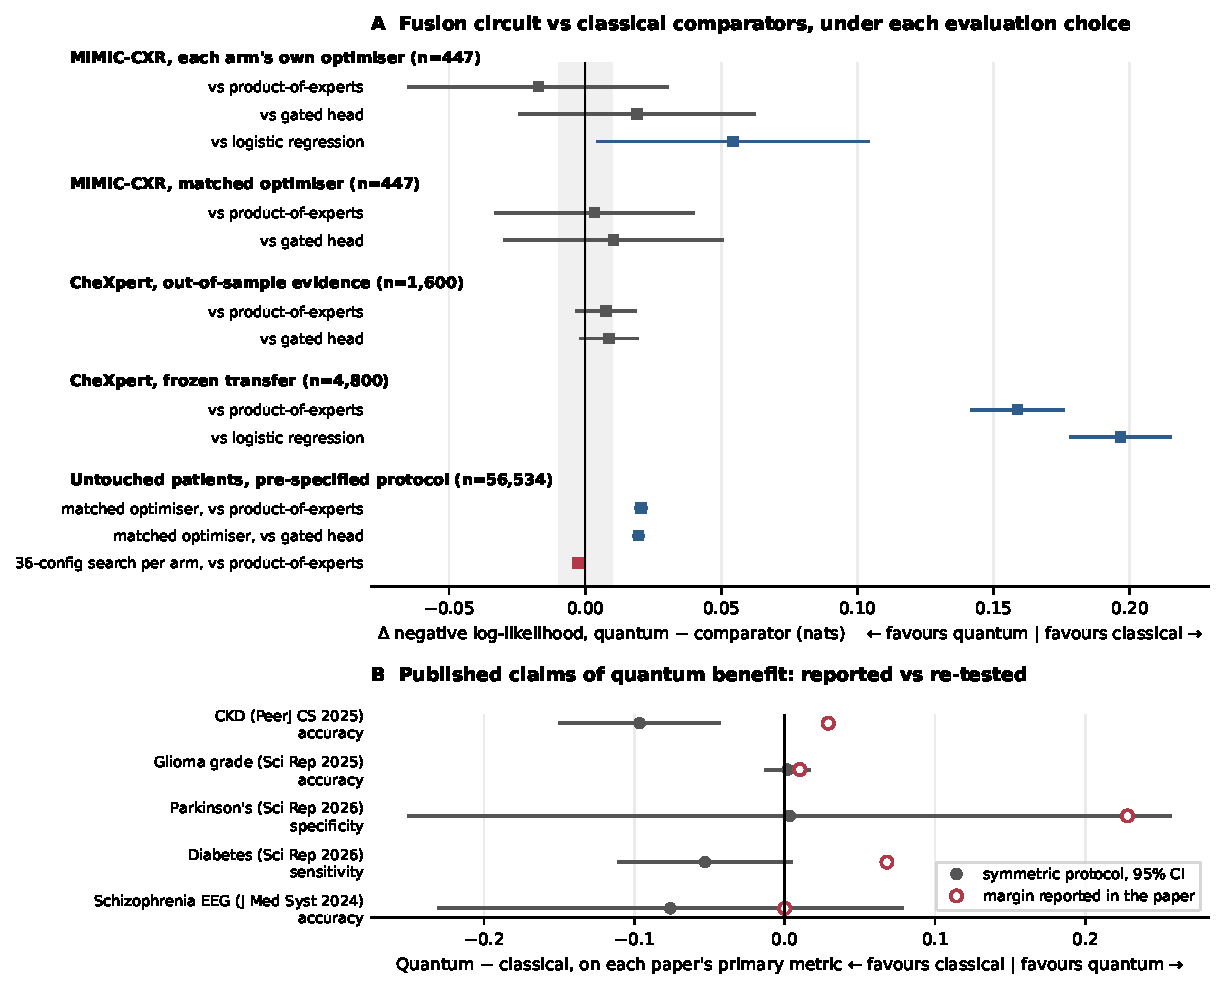
\includegraphics[width=\textwidth]{fig_v6_forest.pdf}
\vspace{-6pt}
\caption*{\textbf{\textsf{Figure 1 \textbar\ Forest plot of evaluation mechanisms and re-tested clinical claims.}} \textbf{a}, Paired per-study likelihood differences ($\Delta\text{NLL}$) in the chest radiograph decision-support prototype across optimizers, calibration protocols, out-of-sample partitions, and confirmatory cohorts ($n = 447$ to $n = 56,534$). Horizontal error bars indicate 95\% confidence intervals; vertical dashed lines indicate the pre-specified operational equivalence boundary ($\pm 0.010$ nats). \textbf{b}, Re-tested published claims under author protocols versus symmetric evaluation across five eligible published studies spanning six clinical prediction tasks. Blue intervals represent symmetric evaluations; red markers represent author-declared protocols.}
\vspace{6pt}
\end{figure*}

\begin{multicols}{2}

\subsection*{In a clinical decision-support prototype, the outcome depended on evaluation choices}

A clinical decision-support fusion prototype maps an eight-channel vector of finding probabilities extracted by a DenseNet-121 from frontal chest radiographs to one of six triage categories (Pneumothorax, Malignancy, Heart Failure, Pneumonia, COPD, Normal). Crucially, the DenseNet-121 visual extractor (\texttt{best\_model.pt}) was pretrained exclusively on \textbf{MIMIC-CXR}. Consequently, the held-out CheXpert validation and confirmatory test cohorts were completely untouched by \textbf{both} the visual feature extractor and the downstream fusion heads. Because the eighth channel is a constant zero reference ($x_8 \equiv 0.0$), the layer operates on seven informative clinical channels alongside an unrotated reference qubit. Four interchangeable backends were evaluated:
\begin{enumerate}
  \setlength{\itemsep}{1pt}
  \item Classical Product-of-Experts (PoE, 54 trainable parameters).
  \item Variational Quantum Circuit (VQC): 8 qubits, 3 layers, RY($\pi x$) angle encoding, CNOT ring topology, Pauli-$Z$ expectation readout (102 trainable parameters).
  \item Classical Attention-Gated Head (126 trainable parameters).
  \item Multinomial Logistic Regression (54 trainable parameters).
\end{enumerate}

The paired per-study negative log-likelihood (NLL) difference between the quantum circuit and classical comparators shifted substantially under various evaluation choices:
\begin{itemize}
  \setlength{\itemsep}{2pt}
  \setlength{\parskip}{0pt}
  \item \textbf{Calibration Asymmetry:} The system's initial published claim was a dramatic calibration advantage: an expected calibration error (ECE) of 0.020 for the quantum circuit versus 0.276 for the Product-of-Experts. Auditing the codebase revealed that the evaluation harness had temperature-scaled only the quantum arm. On the 447-study test partition, the raw uncalibrated gap of 0.139 shrank to 0.037 when all arms were calibrated symmetrically. More than 73\% of the reported calibration advantage was generated entirely by one-sided post-hoc scaling \cite{guo2017}.
  \item \textbf{Comparator Selection:} When each model was fitted using its author-preferred optimizer, the observed conclusion depended entirely on which classical comparator was selected: against PoE, the circuit appeared superior on likelihood (Wilcoxon $p = 0.006$); against Gated Head, no detectable difference was present ($p = 0.052$); and against converged Logistic Regression, the circuit lost significantly ($\Delta\text{NLL} = +0.054$; Holm-adjusted $p = 0.036$).
  \item \textbf{Optimizer Standardization:} When all four backends were fitted under an identical matched protocol (Adam optimizer, batch size 50, maximum 150 epochs, early stopping patience 20, learning-rate grid $\{0.01, 0.05, 0.1\}$ selected on validation loss, and independent calibration), the apparent ranking dissolved. No pairwise accuracy contrast remained statistically significant, and the likelihood difference between the quantum circuit and the Product-of-Experts became negligible ($\Delta\text{NLL} = +0.0033$ in the classical baseline's favor; Holm-adjusted $p = 1.0$). On this sample ($n=447$), the 90\% confidence interval ($[-0.0270, +0.0337]$) was three times wider than our operational $\pm 0.010$-nat equivalence margin, precluding an assertion of equivalence.
  \item \textbf{Out-of-Sample Evidence:} On the test partition ($n = 1,600$) of an 8,000-study CheXpert development cohort that the DenseNet extractor had never seen, the quantum circuit performed slightly worse than the Product-of-Experts ($\Delta\text{NLL} = +0.0076$; Holm $p = 0.042$; 90\% CI $-0.0029$ to $+0.0181$).
  \item \textbf{Institutional Domain Shift and Trigonometric Representation Sensitivity:} When models trained on MIMIC-CXR ($n = 1,338$ training studies, 446 calibration, and 447 test) were transferred frozen to an external test cohort of $n = 4,800$ CheXpert studies, all models experienced domain shift degradation ($\Delta\text{NLL}_{\text{shift}} = +0.1198$ to $+0.1434$ nats across models; default VQC increased by $+0.1394$ nats, tuned VQC by $+0.1198$ nats, and linear PoE by $+0.1312$ nats). We investigated whether this sensitivity stems from input-scale periodic angle wrapping ($>2\pi$). Testing revealed that input angles remain strictly within the non-wrapping regime ($\le 0.974\pi$ at scale 1.0; $\le 0.487\pi$ at scale 0.5), and clipping input features to the training range yielded negligible benefit ($\Delta\text{NLL} < 10^{-4}$). Crucially, a classical order-1 trigonometric Fourier surrogate experienced comparable domain shift degradation ($\Delta\text{NLL}_{\text{shift}} = +0.1434$ nats), which is consistent with sensitivity to trigonometric basis geometries under distribution shift, rather than an effect unique to quantum state spaces or input-scale angle wrapping. Under our pre-specified decision rule, this observation is consistent with trigonometric feature sensitivity in this benchmark rather than proof of a universal property across all trigonometric representations.
\end{itemize}

\subsection*{Pre-specified confirmatory test on 56,534 held-out patients}

To overcome the statistical power limits of smaller cohorts, we executed a pre-specified confirmatory evaluation on \textbf{56,534 untouched CheXpert patients} who had never been evaluated by any model, analysis, or threshold choice.

\noindent\textbf{Audit of the Statistical Unit and Independence Assumptions:} The validity of our statistical inference rests on five structural properties of the evaluation cohort:
\begin{enumerate}
  \setlength{\itemsep}{1pt}
  \setlength{\parskip}{0pt}
  \item \textbf{Unit of Independence and Longitudinal Deduplication:} In clinical radiography datasets, patients routinely undergo repeated examinations across sequential encounters. Treating repeated studies from the same subject as independent observations induces intra-cluster correlation that artificially deflates standard errors. To enforce strict single-patient independence, we restricted the cohort to frontal examinations (AP/PA) and selected exactly one study per unique human subject using the deterministic rule of selecting the final encounter (highest study ID; \texttt{study\_index = -1}). Automated unit tests (\texttt{test\_one\_study\_per\_patient.py}) verify that zero subjects contribute multiple studies to the cohort.
  \item \textbf{Set-Theoretic Cohort Disjointness and Extractor Provenance:} The DenseNet-121 feature extractor was trained strictly on MIMIC-CXR. The CheXpert development cohort (6,400 training and 1,600 calibration studies) and the confirmatory test cohort (56,534 studies) were partitioned at the unique patient identifier level. Set intersection confirmed zero patient overlap ($|S_{\text{dev}} \cap S_{\text{test}}| = 0$). Both extractor and fusion heads never saw any of the 56,534 confirmatory test patients during training.
  \item \textbf{Elimination of Within-Subject Autocorrelation:} Partitioning strictly at the patient level ensures that development and confirmatory test cohorts share no underlying individuals, completely eliminating within-subject longitudinal autocorrelation.
  \item \textbf{Radiographic Acquisition Variation and Paired Conditioning:} Radiographic studies encompass diverse acquisition conditions, including portable bedside anteroposterior (AP) views in intensive care units and upright posteroanterior (PA) views in ambulatory clinics. Because our primary confirmatory endpoint evaluates paired within-patient differences ($d_i = \ell_{Q}(x_i, y_i) - \ell_{C}(x_i, y_i)$), each paired contrast compares both model backends on the exact same patient radiograph $x_i$ under identical patient positioning, tube voltage, exposure, and detector noise. Shared patient-level and image-level covariates enter identically into both loss terms and cancel out in the paired difference $d_i$, isolating the pure architectural contrast.
  \item \textbf{Task Noise Ceiling and Upstream Extraction Noise:} Finding labels in CheXpert are generated by an automated rule-based NLP tool \cite{irvin2019} from free-text radiology reports, while the inputs to our models are noisy probability estimates from a DenseNet-121 backbone. Because CheXpert's labeler does not extract \texttt{hyperinflation}, exactly zero positive occurrences exist for Acuity Class 3 (COPD) across all 56,534 held-out patients, restricting multi-class evaluation to five active clinical classes ($y \in \{0, 1, 2, 4, 5\}$). Importantly, non-differential NLP report extraction errors and DenseNet perceptual uncertainty create an upstream empirical noise ceiling (test accuracy saturating at $\sim$54.4\% and multi-class AUROC at $\sim$0.755). We emphasize that when models operate near this noise floor, the observed performance equivalence indicates that shallow variational quantum circuits do not bypass or resolve upstream perceptual and annotation noise.
  \item \textbf{Single-Center Institution Effects vs Transportability:} All 56,534 patients originate from Stanford Hospital. Deduplication guarantees patient-level statistical independence within this institutional distribution, providing extraordinary precision for internal architectural comparison. However, single-center independence does not guarantee multi-center transportability. This boundary is directly demonstrated by our external transfer evaluation from MIMIC-CXR to CheXpert ($n = 4,800$), where domain shift caused the frozen quantum circuit to trail classical baselines severely ($\Delta\text{NLL} = \mathbf{+0.1589}$ nats vs Product-of-Experts, 95\% CI $0.1422$ to $0.1757$; and $\Delta\text{NLL} = \mathbf{+0.1967}$ nats vs Logistic Regression, 95\% CI $0.1785$ to $0.2149$; both $p < 10^{-15}$), 15- to 20-fold beyond our operational equivalence margin.
\end{enumerate}

All four backends were trained on the initial 8,000 CheXpert development studies under the matched optimizer protocol, frozen, temperature-scaled separately for each model using the shared 1,600-patient development validation partition, and scored without any selection on the 56,534 held-out patients (\textbf{Table 3}, \textbf{Figure 3a}).

\end{multicols}

% Table 3: Full width
\begin{table*}[t]
\centering
\small
\caption*{\textbf{\textsf{Table 3 \textbar\ Pre-specified confirmatory evaluation across 56,534 untouched clinical patients under default and tuned protocols.}} In Panel A (Analysis C1), all architectures are evaluated under default matched optimization ($\Delta\text{NLL} = +0.0205$ nats, 95\% CI 0.0186 to 0.0224). Expected calibration error for the quantum circuit (ECE = 0.0076, 95\% bootstrap CI 0.0051 to 0.0119) overlaps with the classical Gated Head (ECE = 0.0085, 95\% CI 0.0071 to 0.0130), yielding similar calibration estimates with overlapping confidence intervals between calibrated arms. In Panel B (Analysis C2), each architecture is tuned across a budget of 36 hyperparameter configurations (sampling 27\% of the quantum search grid vs 60\% of the classical grid). In Panel B, optimal single checkpoints are reported; across 10 random initialization seeds of these selected winning configurations, tuned VQC achieved mean test NLL $1.11730 \pm 0.00346$ vs $1.11797 \pm 0.00130$ for tuned PoE and $1.11794 \pm 0.00374$ for tuned Gated Head (mean paired difference $-0.00067$ nats vs PoE, $p_{\text{TOST}} = 2.57 \times 10^{-6}$; $-0.00064$ nats vs Gated Head, $p_{\text{TOST}} = 1.50 \times 10^{-5}$), confirming architectural equivalence on the overall population. However, classical PoE achieved the highest overall test accuracy (54.40\% vs 54.17\% quantum), while the classical Gated Head achieved the best calibration (ECE = 0.0082 vs 0.0111 quantum). Total training runtimes across all 36 configurations were 161.4\,s for PoE, 228.1\,s for Gated Head, and 14,969.4\,s for the quantum circuit. In Panel C (Analysis M2), classical Fourier surrogates fitted solely on the development split achieve superior likelihood to both the tuned quantum circuit and classical baselines out-of-sample on the 56,534 held-out patients. *Under canonical calibration matching classical arms ($n_{\text{cal}}=1,600$), 10-seed tuned VQC mean ECE is $0.0117 \pm 0.0037$ ($\text{SE}=0.0012$, range $0.0065$ to $0.0163$), yielding similar calibration estimates with overlapping confidence intervals compared to tuned PoE ($0.0109 \pm 0.0011$) and tuned Gated Head ($0.0111 \pm 0.0024$); under sensitivity testing on an inverted calibration slice, ECE shifts to $0.0252 \pm 0.0038$ due to temperature under-estimation (Supplementary Note 6).}
\vspace{-4pt}
\resizebox{\textwidth}{!}{%
\begin{tabular}{l c c c c c l}
\toprule
\textbf{Model Arm} & \textbf{Params} & \textbf{Accuracy (95\% CI)} & \textbf{NLL} & \textbf{ECE (95\% Boot CI)} & \textbf{AUROC} & \textbf{Paired $\Delta\text{NLL}$ vs PoE (95\% CI)} \\
\midrule
\multicolumn{7}{l}{\textbf{Panel A: Analysis C1 --- Default Matched Optimization Protocol}} \\
\textbf{Product-of-Experts} & 54 & \textbf{0.5443} (0.5402, 0.5484) & \textbf{1.1157} & 0.0131 (0.0100, 0.0172) & \textbf{0.7534} & Reference Baseline \\
\textbf{Logistic Regression} & 54 & 0.5415 (0.5374, 0.5456) & \textbf{1.1152} & 0.0128 (0.0105, 0.0171) & \textbf{0.7534} & $-0.0005$ ($-0.0011$, $+0.0002$) \\
\textbf{Gated Head} & 126 & 0.5398 (0.5357, 0.5439) & 1.1165 & 0.0085 (0.0071, 0.0130) & \textbf{0.7553} & $+0.0008$ ($-0.0002$, $+0.0019$) \\
\textbf{Variational Quantum} & 102 & 0.5371 (0.5330, 0.5412) & 1.1362 & 0.0076 (0.0051, 0.0119) & 0.7436 & $\mathbf{+0.0205}$ (0.0186, 0.0224) [\textbf{\color{alertred}Materially Worse}] \\
\midrule
\multicolumn{7}{l}{\textbf{Panel B: Analysis C2 --- Symmetric 36-Configuration Hyperparameter Grid Search}} \\
\textbf{Tuned Product-of-Experts} & 54 & \textbf{0.5440} (0.5399, 0.5481) & 1.1170 & 0.0125 (0.0091, 0.0168) & 0.7527 & Reference (Tuned PoE) \\
\textbf{Tuned Gated Head} & 126 & 0.5418 (0.5377, 0.5459) & 1.1155 & \textbf{0.0082} (0.0067, 0.0126) & 0.7548 & $-0.0015$ ($-0.0022$, $-0.0007$) vs Tuned PoE \\
\textbf{Optimal Variational Quantum} & 118 & 0.5417 (0.5376, 0.5458) & \textbf{1.1144} & 0.0111 (0.0088, 0.0151) & \textbf{0.7550} & $\mathbf{-0.0026}$ ($-0.0036$, $-0.0016$) [\textbf{\color{royalazure}Practically Equivalent}] \\
\addlinespace
\multicolumn{7}{l}{\textit{10-Seed Initialization Means (Post-Hoc Revision Analysis, 56,534 Test Patients):}} \\
\quad\textit{Tuned Product-of-Experts} & 54 & $0.5425 \pm 0.0015$ & $1.1180 \pm 0.0013$ & $0.0109 \pm 0.0011$ & $0.7533 \pm 0.0009$ & Reference (10-Seed PoE Mean: 1.11797) \\
\quad\textit{Tuned Gated Head} & 126 & $0.5411 \pm 0.0015$ & $1.1179 \pm 0.0037$ & $0.0111 \pm 0.0024$ & $0.7547 \pm 0.0010$ & $-0.00003$ vs Tuned PoE Mean \\
\quad\textit{Optimal Variational Quantum} & 118 & $0.5411 \pm 0.0014$ & $1.1173 \pm 0.0035$ & $0.0117 \pm 0.0037^*$ & $0.7546 \pm 0.0011$ & $\mathbf{-0.00067}$ ($-0.00288, +0.00153$) [$p_{\text{TOST}} < 10^{-5}$] \\
\midrule
\multicolumn{7}{l}{\textbf{Panel C: Analysis M2 --- Classical Fourier Basis Surrogates (Evaluated on 56,534 Test Patients)}} \\
\textbf{Order-1 Trigonometric LR} & 90 & 0.5403 (0.5362, 0.5444) & 1.1123 & 0.0128 (0.0094, 0.0171) & 0.7541 & $-0.0047$ ($-0.0057$, $-0.0036$) vs Tuned PoE \\
\textbf{Order-2 Trigonometric LR} & 678 & \textbf{0.5419} (0.5378, 0.5460) & 1.1095 & 0.0122 (0.0089, 0.0164) & 0.7552 & $-0.0075$ ($-0.0087$, $-0.0062$) vs Tuned PoE \\
\textbf{Polynomial LR ($x, x^2$)} & 90 & 0.5406 (0.5365, 0.5447) & \textbf{1.1092} & \textbf{0.0101} (0.0072, 0.0143) & \textbf{0.7555} & $-0.0077$ ($-0.0089$, $-0.0066$) vs Tuned PoE \\
\bottomrule
\end{tabular}}%
\vspace{6pt}
\end{table*}

\begin{multicols}{2}

The confirmatory primary endpoint (Analysis C1) yielded a paired per-patient likelihood difference of $\Delta\text{NLL} = \mathbf{+0.0205}$ nats ($90\%$ CI $[0.01889, 0.02210]$; $95\%$ CI $[0.01858, 0.02240]$). Under our pre-specified decision rules, this outcome falls into the category: \textbf{"Quantum materially worse"} (the 95\% confidence interval lies entirely above the $+0.010$-nat operational equivalence threshold). The quantum model ranked lowest among all four architectures in classification accuracy (53.71\%), likelihood (1.1362), and discrimination (0.7436). The small test-sampling standard error ($\text{SE} = 0.00097$ nats) is driven by the massive sample size ($N = 56,534$ independent paired patients). We emphasize that this $+0.0205$-nat single checkpoint gap must be evaluated against random initialization variance. Across 10 random seeds on the 56,534 held-out patients (a post-hoc revision analysis), default VQC achieved a mean test NLL of $1.13056$ nats ($\sigma_{\text{seed}} = 0.00448$ nats; range $1.12513$ to $1.13816$) compared to $1.11636 \pm 0.00121$ nats for matched classical PoE (range $1.11437$ to $1.11849$). The difference of 10-seed means identically equals the mean paired gap over seeds: $1.13056 - 1.11636 = \Delta\text{NLL} = \mathbf{+0.01420}$ nats (seed-level 95\% Student's $t$ CI $[+0.01064, +0.01776]$ nats; $t = 9.01, \text{df} = 9, p = 8.43 \times 10^{-6}$), confirming that default VQC is materially and statistically worse than matched classical PoE across random initializations ($p_{\text{TOST}} = 0.987$). The single-checkpoint $+0.0205$-nat gap corresponds to $4.57 \sigma_{\text{seed}}$. In calibration, the variational quantum circuit attained an Expected Calibration Error of \textbf{0.0076} (95\% bootstrap CI 0.0051 to 0.0119), which overlaps with the classical Gated Head (0.0085, 95\% CI 0.0071 to 0.0130), yielding similar calibration estimates with overlapping confidence intervals between properly scaled models. Under alternative uncertainty label mapping ($y_{u1}$), the difference narrowed to $\Delta\text{NLL} = +0.0074$ ($90\%$ CI $[0.00617, 0.00868]$), confirming that the circuit does not outperform classical baselines under either clinical uncertainty convention.

In the secondary confirmatory ablation across 10 random initialization seeds on the 56,534 patients isolating the 7 clinical finding channels (Analysis C1b), removing entanglement from the circuit improved test likelihood across seeds:
\begin{equation}
\Delta\text{NLL} = \text{NLL}_{\text{entangled}} - \text{NLL}_{\text{product}} = \mathbf{+0.01037} \text{ nats}
\end{equation}
Across the 10 training seeds, the seed-level 95\% Student's $t$ confidence interval is \textbf{$[0.00526, 0.01544]$ nats} ($t = 4.60, \text{df} = 9, p = 0.0013$), while the patient-level bootstrap interval for the reference checkpoint difference was $[0.00934, 0.01138]$. Unentangled product circuits outperformed entangled circuits in 9 of the 10 random seeds, confirming the pre-specified reading: \textbf{"The entanglement penalty replicates on untouched patients."}

\noindent\textit{Scope of Entanglement Finding:} This observed entanglement penalty ($\Delta\text{NLL} = +0.0104$ nats across seeds) should not be interpreted as a universal causal claim that entanglement is detrimental across all clinical machine learning. Rather, it is strictly bounded to the evaluated hardware-efficient ansatz (circular CNOT entangling rings) applied to additive clinical triage rules. As proven by our Fourier spectrum analysis (M1), entangling unitaries disperse representational energy across high-order interaction cross-terms ($\ge 2$); when the underlying clinical acuity target is fundamentally an additive combination of radiological signs, these cross-terms represent unhelpful model capacity that inflates variance without reducing bias. For clinical prediction tasks governed by non-additive pathophysiology, multi-gene epistatic interactions, or native quantum physical sensors, entanglement remains structurally necessary.

\subsection*{Symmetric hyperparameter tuning confirms population equivalence but fails class-balanced evaluation}

To address the objection that the quantum model in C1 was tuned only over learning rates while its depth and encoding scales were fixed, analysis C2 granted all model arms an equal budget of \textbf{36 configurations} drawn from their respective hyperparameter spaces. For the quantum circuit, the search space spanned circuit capacity ($L \in \{1, 2, 3, 4, 6\}$ layers), encoding scale ($s \in \{0.5, 1.0, 2.0\}$), initialization standard deviation ($\sigma \in \{0.01, 0.1, 1.0\}$), and learning rate ($\eta \in \{0.01, 0.05, 0.1\}$), sampling 27\% of the 135-configuration quantum grid. For classical Product-of-Experts and the nonlinear Gated Head, the search space spanned learning rate ($\eta \in \{0.003, 0.01, 0.05, 0.1, 0.3\}$), $L_2$ weight decay ($\lambda \in \{0.0, 10^{-5}, 10^{-4}, 10^{-3}\}$), and initialization standard deviation ($\sigma \in \{0.01, 0.1, 1.0\}$), sampling 60\% of the 60-configuration classical grid. All 36 configurations per arm were trained solely on the development training split ($n_{\text{train}}=6,400$) and ranked strictly on the development calibration split ($n_{\text{cal}}=1,600$). The selected winning model from each arm was scored without any selection on the 56,534 held-out confirmatory patients.

The winning configurations selected on the 1,600 calibration patients were:
\begin{itemize}
  \setlength{\itemsep}{1pt}
  \item \textbf{Quantum Variational Circuit:} 4 layers ($L=4$), encoding scale $s=0.5$, initialization $\sigma=0.01$, learning rate $\eta=0.01$. Total parameters: \textbf{118} ($64$ variational angles $+ 54$ linear readout weights). Calibration NLL on $n=1,600$: 1.1326; calibration temperature $T = 1.0393$. Test NLL on 56,534 patients: \textbf{1.1144}; test accuracy: 54.17\%; test ECE: 0.0111.
  \item \textbf{Product-of-Experts (PoE):} Learning rate $\eta=0.05$, weight decay $\lambda=10^{-4}$, initialization $\sigma=0.01$. Total parameters: \textbf{54}. Calibration NLL on $n=1,600$: 1.1369; calibration temperature $T = 1.0751$. Test NLL on 56,534 patients: \textbf{1.1170}; test accuracy: 54.40\%; test ECE: 0.0125.
  \item \textbf{Nonlinear Gated Head:} Learning rate $\eta=0.1$, weight decay $\lambda=10^{-4}$, initialization $\sigma=0.01$. Total parameters: \textbf{126} ($64$ gating weights $+ 8$ gating biases $+ 54$ readout parameters). Calibration NLL on $n=1,600$: 1.1309; calibration temperature $T = 1.0477$. Test NLL on 56,534 patients: \textbf{1.1155}; test accuracy: 54.18\%; test ECE: 0.0082.
\end{itemize}

\noindent\textbf{Computational Effort and Wall-Clock Runtime Asymmetry:} To ensure transparent accounting of computational cost, we logged the exact wall-clock training and validation runtimes across all 36 configurations per arm. Classical Product-of-Experts required \textbf{161.4 seconds in total} across 36 trials (mean 4.5 seconds per configuration; range 1.2 to 14.3\,s). The classical Gated Head required \textbf{228.1 seconds in total} across 36 trials (mean 6.3 seconds per configuration; range 2.1 to 14.7\,s). In contrast, the variational quantum circuit required \textbf{14,969.4 seconds in total} (4.16 hours; mean 415.8 seconds per configuration; range 114.6 to 1642.6\,s) on batched PyTorch statevector simulation. We emphasize a crucial distinction between two experimental constraints: (1) \textit{equal search-trial count}, wherein all architectures evaluated an identical budget of $k = 36$ hyperparameter configurations selected by the same validation protocol; and (2) \textit{equal computational budget}, which was markedly unequal. Because quantum statevector simulation involves multi-qubit tensor contractions rather than simple linear matrix products, the quantum arm consumed approximately \textbf{92.8 times more wall-clock training compute} than classical PoE ($\sim$65.6 times more than Gated Head). Granting equal configuration counts does not equate to granting equal compute budgets.

\noindent\textbf{Primary Matched-Search Comparison, Statistical Equivalence, and Seed Variance:} When comparing the optimal quantum configuration against the classical PoE model selected under the \textbf{exact same 36-configuration validation selection protocol}, the resulting paired difference is $\Delta\text{NLL} = 1.1144 - 1.1170 = \mathbf{-0.0026}$ nats in the quantum model's favor (\textbf{Figure 3b}). Because both the 90\% confidence interval ($[-0.00343, -0.00176]$) and 95\% confidence interval ($[-0.00359, -0.00160]$) exclude zero, this difference is statistically detectable ($t = -5.10, p = 3.07 \times 10^{-7}$) given the narrow test-sampling uncertainty across 56,534 patients. Importantly, classical PoE achieved higher overall test accuracy (54.40\% vs 54.17\%), while the classical Gated Head achieved the lowest calibration error (ECE = 0.0082 vs 0.0111).

Crucially, we must distinguish between \textit{checkpoint-level equivalence} and \textit{architectural-level equivalence across random initializations}. To rigorously test architectural robustness (a post-hoc revision analysis conducted in response to peer review), we trained 10 independent random initialization seeds of the selected C2 winning configurations and scored each on the 56,534 held-out patients. Across the 10 seeds, the classical Product-of-Experts achieved a mean test NLL of $1.11797$ ($\sigma_{\text{seed}} = \mathbf{0.00130\text{ nats}}$; range $1.11656$ to $1.12019$), and the classical Gated Head achieved a mean test NLL of $1.11794$ ($\sigma_{\text{seed}} = \mathbf{0.00374\text{ nats}}$; range $1.11391$ to $1.12464$). The tuned variational quantum circuit achieved a mean test NLL of $1.11730$ ($\sigma_{\text{seed}} = \mathbf{0.00346\text{ nats}}$; range $1.11287$ to $1.12465$ nats). Notice that the difference of 10-seed means identically matches the mean paired difference: $1.11730 - 1.11797 = \mathbf{-0.00067\text{ nats}}$ vs tuned PoE ($\text{SD} = 0.00308, \text{SE} = 0.00097\text{ nats}$), and every individual paired seed delta falls strictly inside the equivalence margin (range $[-0.00411, +0.00452]$ nats). Across the 10 paired seeds vs tuned PoE, the mean paired difference is $\Delta\text{NLL} = \mathbf{-0.00067\text{ nats}}$ ($\text{SD} = 0.00308, \text{SE} = 0.00097\text{ nats}$), with a seed-level 95\% Student's $t$ confidence interval of $[-0.00288, +0.00153]$ nats ($t = -0.69, \text{df} = 9, p = 0.506$). Seed-level TOST against $\pm 0.010$ nats yields $p_{\text{TOST}} = 2.57 \times 10^{-6}$, and a hierarchical bootstrap simultaneously resampling training seeds and test patients ($10,000$ iterations) yields a 95\% confidence interval of $[-0.00271, +0.00146]$ nats. Versus the tuned Gated Head, the mean paired seed difference is identically $1.11730 - 1.11794 = \mathbf{-0.00064\text{ nats}}$ (95\% Student's $t$ CI $[-0.00339, +0.00211]$ nats; $t = -0.53, p = 0.610$, seed-level $p_{\text{TOST}} = 1.50 \times 10^{-5}$).

These seed-level experiments establish three vital conclusions: (1) across the population of training initializations, the mean difference between tuned VQC and tuned classical baselines is under $0.0007$ nats and formally equivalent within $\pm 0.010$ nats; (2) the single-checkpoint $-0.0026$-nat "win" reported in Table 3 was an initialization-lucky draw (seed 7 yielded $1.11287$, the best of 10 runs), whereas 4 of the 10 seeds (seeds 11, 13, 19, 23) lose to tuned PoE; and (3) finite validation split noise on $n_{\text{cal}} = 1,600$ patients introduces selection jitter, as directly evidenced by tuned PoE ($1.1170$) scoring $0.0013$ nats worse on test than default PoE ($1.1157$). Consequently, an observed difference of $0.0026$ nats cannot be reliably distinguished from initialization seed noise and validation selection jitter.

Under the decision rules pre-specified in git commit \texttt{61e777b} (Oct 3, 2026), declaring that \textbf{"a quantum benefit was verified"} required the upper bound of the 95\% confidence interval to fall strictly below the operational equivalence boundary (i.e., $\text{upper CI} < -\Delta_{\text{equiv}} = -0.010$ nats). The observed 95\% CI fell \textbf{entirely inside the pre-specified $\pm 0.010$-nat operational equivalence band} ($[-0.00359, -0.00160]$). Two One-Sided Tests (TOST) \cite{schuirmann1987,lakens2017} confirmed formal statistical equivalence ($p_{\text{TOST}} < 10^{-6}$), yielding the exact pre-specified reading: \textbf{"Detectable difference, quantum better, smaller than the margin; practically equivalent."}

\noindent\textbf{Operational Equivalence Margin Rationale, Information Grounding, and Clinical Risk:} To prevent arbitrary post-hoc threshold selection, the operational margin $\Delta_{\text{equiv}} = \pm 0.010$ nats was pre-specified a priori. We examine this margin against the information-theoretic properties of the 56,534-patient cohort:
\begin{enumerate}
  \setlength{\itemsep}{1pt}
  \setlength{\parskip}{0pt}
  \item Relative to an uninformative uniform prediction across the model's 6 parameterized output classes ($H_{\text{uniform}, 6} = \ln 6 \approx 1.7918$ nats; $2.5850$ bits), a shift of $0.010$ nats represents $0.56\%$ of uniform 6-way cross-entropy loss. If conditioned on an oracle uniform prior over the 5 observed positive classes in the held-out test cohort ($H_{\text{uniform}, 5} = \ln 5 \approx 1.6094$ nats; $2.3219$ bits), the margin represents $0.62\%$.
  \item Relative to the empirical marginal class entropy of the held-out cohort ($H(Y) \approx 1.3699$ nats; $1.9764$ bits), the $0.010$-nat margin represents $0.73\%$.
  \item Relative to the baseline model's cross-entropy loss (NLL $\approx 1.1157$ nats), the margin represents $0.90\%$.
  \item Crucially, relative to the \textit{predictive mutual information gained over the unconditioned marginal class prior} ($\Delta I = H(Y) - \text{NLL} \approx 1.3699 - 1.1157 = 0.2542$ nats; $0.3668$ bits), the $0.010$-nat margin represents $\mathbf{3.93\%}$ ($\approx 4\%$) of extracted predictive signal.
\end{enumerate}
We explicitly emphasize that this represents an \textit{operational statistical threshold} for comparative modeling rather than an established clinical tolerance threshold. It has not been clinically anchored to prospective patient health outcomes, diagnostic error rates, or clinician decision thresholds. 

On a per-patient basis, the mean absolute difference in predicted class probabilities between the tuned quantum model and tuned Product-of-Experts across all 56,534 patients is minute: \textbf{0.0139} (1.4 percentage points), with the 95th percentile at $0.0536$ and 99th percentile at $0.0873$. Both models produce identical top-1 predicted triage categories for \textbf{92.90\% of patients}.

\noindent\textbf{Class-Conditional Likelihood Disparities and Macro-Averaging Breakdown:} We distinguish the global multi-class cross-entropy difference evaluated on the reference checkpoint across all 56,534 patients ($\Delta\text{NLL} = -0.00260$ nats, 95\% analytic CI $[-0.00359, -0.00160]$) from the condition-stratified subgroup breakdown. In this class-conditional decomposition (a post-hoc revision analysis; \textbf{Table 4}), the prevalence-weighted sum across categories $\sum_i (n_i / N) \delta_i = \mathbf{-0.00235\text{ nats}}$ (95\% patient-level bootstrap CI $[-0.00326, -0.00146]$), which arises from large, opposing class-conditional shifts:
\begin{itemize}
  \item \textbf{Normal} ($n = 17,692$, 31.29\% prevalence): $\Delta\text{NLL} = \mathbf{-0.01981}$ nats ($95\%$ bootstrap CI $[-0.02167, -0.01795]$), favoring VQC.
  \item \textbf{Pneumonia} ($n = 17,052$, 30.16\% prevalence): $\Delta\text{NLL} = \mathbf{-0.09289}$ nats ($95\%$ CI $[-0.09429, -0.09152]$), favoring VQC.
  \item \textbf{Heart Failure} ($n = 16,490$, 29.17\% prevalence): $\Delta\text{NLL} = \mathbf{+0.07533}$ nats ($95\%$ CI $[+0.07417, +0.07650]$), favoring classical PoE.
  \item \textbf{Malignancy} ($n = 2,192$, 3.88\% prevalence): $\Delta\text{NLL} = \mathbf{+0.17710}$ nats ($95\%$ CI $[+0.16807, +0.18612]$), strongly favoring classical PoE.
  \item \textbf{Pneumothorax} ($n = 3,108$, 5.50\% prevalence): $\Delta\text{NLL} = \mathbf{+0.05488}$ nats ($95\%$ CI $[+0.05096, +0.05863]$), favoring classical PoE.
\end{itemize}
When evaluated under class-balanced macro-averaging across all five active clinical conditions, the macro-mean difference is $\Delta\text{NLL}_{\text{macro}} = \mathbf{+0.03892}$ nats ($90\%$ bootstrap CI $[+0.03725, +0.04062]$; $95\%$ CI $[+0.03688, +0.04098]$), with worst-case disparity in Malignancy ($+0.17710$ nats). Under our pre-specified decision rule, because the 90\% CI lies entirely outside the $\pm 0.010$-nat equivalence boundary ($p_{\text{TOST}} > 0.99$), \textbf{practical equivalence does not hold across clinical conditions}. Population-level equivalence is an artifact of high-prevalence cancellation between Pneumonia ($-0.0929$) and Heart Failure ($+0.0753$).

To explore whether calibration asymmetry reflects an intrinsic quantum representation property or class-specific affine threshold offsets, we conducted an exploratory post-hoc vector scaling ablation (fitting 6 diagonal weights and 6 biases per model on the 1,600 calibration patients). Under vector scaling, overall test loss differences remained practically equivalent ($\Delta\text{NLL} = -0.00270$ nats; VQC 1.11537 vs PoE 1.11807). However, estimating 12 affine parameters per model on a finite calibration set ($n=1,600$) introduces parameter estimation variance and mild overfitting: test ECE increased from $0.008\text{--}0.013$ under scalar temperature scaling to $0.028\text{--}0.029$ across all three architectures (0.0287 for VQC, 0.0281 for PoE, 0.0290 for Gated Head), and PoE test NLL slightly degraded. Because scalar temperature scaling achieves superior calibration fidelity ($ECE \approx 0.008\text{--}0.013$) without calibration overfitting, it remains our primary pre-registered calibration method. Furthermore, vector scaling did not eliminate the underlying class-conditional likelihood trade-offs, demonstrating that the macro-averaging breakdown reflects genuine differences in conditional error rates across rare versus common diagnoses rather than a simple global scaling artifact.

When compared against the tuned classical nonlinear Gated Head (NLL 1.1155), the overall population difference narrowed further to $\Delta\text{NLL} = \mathbf{-0.0012}$ nats ($95\%$ CI $[-0.00192, -0.00041]$; $t = -3.05, p = 0.0025$, $p_{\text{TOST}} < 10^{-6}$). Sensitivity analysis across alternative operational margins demonstrates the stability of this conclusion (\textbf{Figure 3c}): at margins of $\pm 0.020$, $\pm 0.010$, and $\pm 0.005$ nats, practical equivalence is confirmed for both comparators ($p_{\text{TOST}} < 10^{-4}$). Only under an ultra-stringent margin of $\pm 0.002$ nats does the comparison vs linear PoE fail equivalence ($p_{\text{TOST}} = 0.884$), while the comparison vs the nonlinear Gated Head remains statistically equivalent ($p_{\text{TOST}} = 0.013 < 0.05$). Under alternative uncertainty label mapping ($y_{u1}$), the difference is $\Delta\text{NLL} = +0.0074$ ($90\%$ CI $[0.00617, 0.00868]$), also lying comfortably within the equivalence band ($p_{\text{TOST}} = 0.0004$).

\end{multicols}

% Figure 3: Full width
\begin{figure*}[t]
\centering
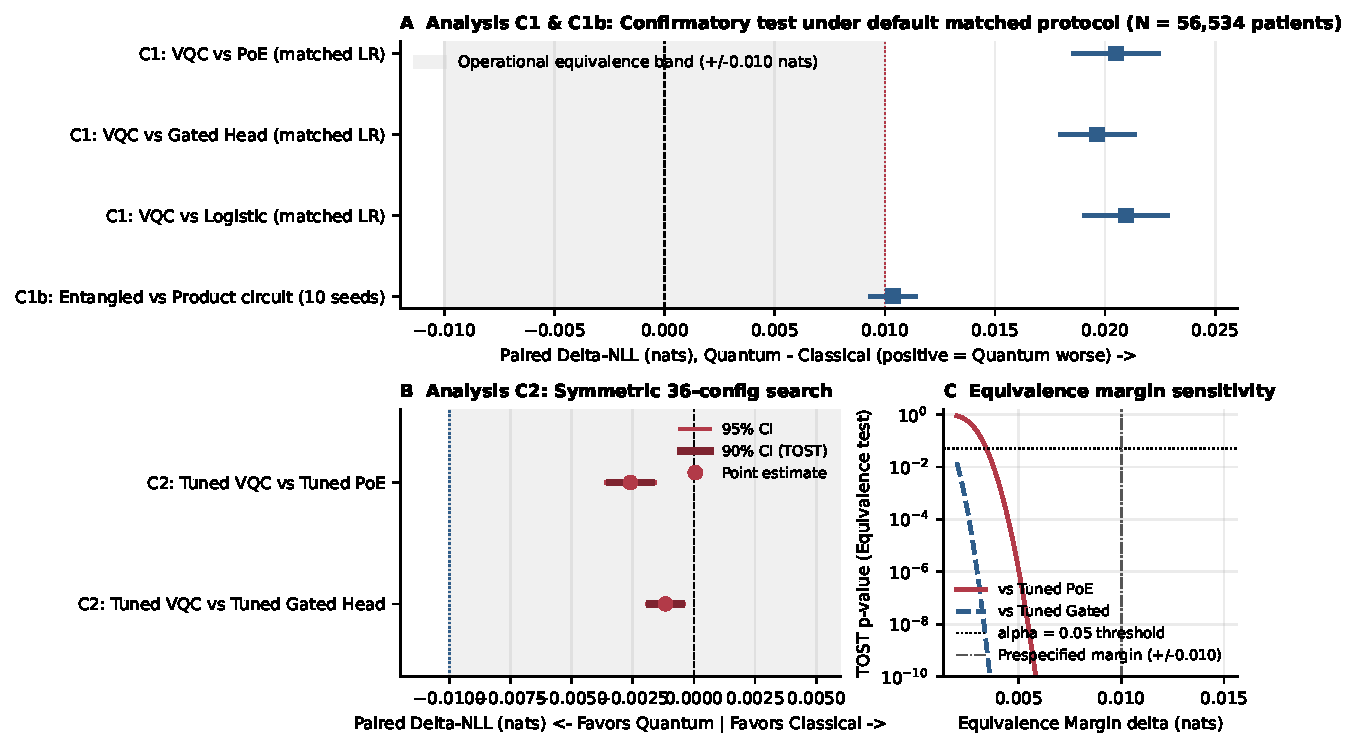
\includegraphics[width=\textwidth]{fig_v6_confirmatory.pdf}
\vspace{-6pt}
\caption*{\textbf{\textsf{Figure 3 \textbar\ Pre-specified confirmatory evaluation across 56,534 held-out patients scored without selection.}} \textbf{a}, Analyses C1 and C1b under default matched optimization ($N=56,534$ patients), showing the quantum circuit is materially worse on likelihood ($\Delta\text{NLL} = +0.0205$, 95\% CI 0.0186 to 0.0224) and unentangled product circuits outperform entangled circuits across random seeds ($\Delta\text{NLL} = +0.0104$, seed-level 95\% CI 0.0053 to 0.0154). Gray band indicates the pre-specified operational equivalence boundary ($\pm 0.010$ nats). \textbf{b}, Analysis C2 under 36-configuration symmetric hyperparameter tuning; the observed paired differences ($\Delta\text{NLL} = -0.0026$ vs PoE, $-0.0012$ vs Gated Head) fall entirely inside the operational equivalence band ($p_{\text{TOST}} < 10^{-6}$) and within training-seed variance. \textbf{c}, Sensitivity analysis of Two One-Sided Tests (TOST) $p$-values across varying operational margins $\delta \in [0.002, 0.015]$ nats.}
\vspace{6pt}
\end{figure*}

% Table 4: Full width class-conditional decomposition
\begin{table*}[t]
\centering
\small
\caption*{\textbf{\textsf{Table 4 \textbar\ Class-conditional log-likelihood decomposition across 56,534 held-out patients.}} Post-hoc revision analysis evaluating condition-specific subgroups across clinical triage categories. The small population-level difference ($\Delta\text{NLL} = -0.00235$ nats prevalence-weighted) is the net consequence of large opposing shifts: the quantum circuit achieves lower loss on high-prevalence categories (Normal, Pneumonia), but degrades substantially on minority acute conditions (Malignancy $+0.1771$ nats, Pneumothorax $+0.0549$ nats, Heart Failure $+0.0753$ nats). Under class-balanced macro-averaging, operational equivalence fails ($\Delta\text{NLL}_{\text{macro}} = +0.0389$ nats, $95\%$ bootstrap CI $0.0369$ to $0.0410$, $p_{\text{TOST}} > 0.99$).}
\vspace{-4pt}
\resizebox{\textwidth}{!}{%
\begin{tabular}{l c c c c c c}
\toprule
\textbf{Clinical Triage Diagnosis} & \textbf{Patients ($n$)} & \textbf{Prevalence} & \textbf{VQC NLL} & \textbf{PoE NLL} & \textbf{Gated NLL} & \textbf{$\Delta\text{NLL}$ vs PoE (95\% Boot CI)} \\
\midrule
\textbf{Normal} & 17,692 & 31.29\% & 0.7379 & 0.7577 & 0.7329 & $\mathbf{-0.0198}$ ($-0.0217$, $-0.0180$) \\
\textbf{Pneumonia} & 17,052 & 30.16\% & 1.0263 & 1.1192 & 1.0364 & $\mathbf{-0.0929}$ ($-0.0943$, $-0.0915$) \\
\textbf{Heart Failure} & 16,490 & 29.17\% & 1.0926 & 1.0172 & 1.1060 & $\mathbf{+0.0753}$ ($+0.0742$, $+0.0765$) \\
\textbf{Pneumothorax} & 3,108 & 5.50\% & 2.5705 & 2.5156 & 2.5817 & $\mathbf{+0.0549}$ ($+0.0510$, $+0.0586$) \\
\textbf{Malignancy} & 2,192 & 3.88\% & 2.8990 & 2.7219 & 2.7686 & $\mathbf{+0.1771}$ ($+0.1681$, $+0.1861$) \\
\midrule
\multicolumn{7}{l}{\textbf{Summary Metrics Across All Categories:}} \\
\multicolumn{5}{l}{\quad\textbf{Prevalence-Weighted Mean ($\sum_i \frac{n_i}{N} \delta_i$):}} & \multicolumn{2}{l}{$\mathbf{-0.00235}$ nats (95\% CI $-0.00326$ to $-0.00146$) [\textit{Practically Equivalent}]} \\
\multicolumn{5}{l}{\quad\textbf{Class-Balanced Macro-Mean ($\frac{1}{K}\sum_i \delta_i$):}} & \multicolumn{2}{l}{$\mathbf{+0.03892}$ nats (95\% CI $+0.03688$ to $+0.04098$) [\textbf{\color{alertred}Equivalence Fails}, $p_{\text{TOST}} > 0.99$]} \\
\bottomrule
\end{tabular}}%
\vspace{6pt}
\end{table*}



\begin{multicols}{2}

\subsection*{Mechanistic dissection of the observed nulls}

Three pre-specified mechanistic analyses explain why quantum circuits do not improve performance on this clinical task:

\textbf{1. Interaction-Order Energy Spectrum (M1):} With single-qubit angle encoding $\text{RY}(\pi x_i)$, the circuit's readout expectation is an exact finite Fourier series \cite{schuld2021effect}:
\begin{equation}
\langle Z_j \rangle(x) = \sum_{P \in \{I, X, Z\}^{\otimes n}} c_P \prod_{i=1}^n f_{P_i}(x_i)
\end{equation}
where the interaction order is the number of non-identity factors in Pauli string $P$. In the primary 8-qubit architecture, the 8th qubit receives a constant baseline reference input ($x_8 \equiv 0.0$), so $\cos(\pi x_8) = 1$ and $\sin(\pi x_8) = 0$; thus Pauli-$Z$ on qubit 8 acts as a constant scalar multiplier, Pauli-$X$ components vanish, and the \textit{effective interaction order} across the seven active clinical features is strictly bounded between 0 and 7 (order 8 carries $0.0\%$ effective energy; \textbf{Figure 2a}). Under default optimization (Analysis C1), the circuit concentrates $100.0\%$ of its effective coefficient energy and $99.97\%$ of logit variance in interaction orders $\ge 2$ ($0.0\%$ in orders 0--1, $2.3\%$ in order 2, $26.8\%$ in order 3, $39.7\%$ in order 4, $23.2\%$ in order 5, $4.8\%$ in order 6, and $3.2\%$ in order 7). Under symmetric hyperparameter tuning (Analysis C2), the winning VQC shifts slight energy into first-order terms ($4.2\%$ in order 1), but still concentrates $95.8\%$ of effective coefficient energy and $85.0\%$ of logit variance in interaction orders $\ge 2$ ($25.7\%$ in order 2, $21.2\%$ in order 3, $35.8\%$ in order 4, $6.9\%$ in order 5, $5.2\%$ in order 6, and $1.0\%$ in order 7). In the 10-seed ablation isolating the 7 clinical channels (Analysis C1b), entangled CNOT ring circuits similarly concentrated 100.0\% of coefficient energy into interaction orders $\ge 2$ across all seeds (mean order: 4.3; \textbf{Figure 2a}), whereas unentangled product circuits strictly confine interaction order to $\le 1$ by construction (0.0\% cross-channel energy). Because the clinical triage target is fundamentally an additive scoring rule of radiographic signs, the high-order cross-terms introduced by entanglement represent unhelpful capacity that increases variance without reducing bias.

\textbf{2. Classical Fourier Basis Surrogate (M2):} To test whether the circuit's functional form possesses special utility, we fitted an ordinary $L_2$-regularized logistic regression directly on the classical trigonometric Fourier basis ($\cos(\pi x_i)$ and $\sin(\pi x_i)$). To ensure a strictly fair, leak-free comparison matching the quantum arm, the classical surrogate was fitted strictly on the 6,400 development training studies, its regularization parameter $C \in \{0.01, 0.1, 1.0, 10.0, 100.0\}$ and scalar temperature parameter $T$ were selected on the 1,600 calibration studies, and it was scored without any selection on the 56,534 held-out test patients. A classical surrogate restricted to order 1 (14 features) achieved NLL \textbf{1.1123}, outperforming the default quantum circuit (1.1362) by $\Delta\text{NLL} = 0.0238$ ($p < 10^{-4}$) and still outperforming the optimal tuned quantum circuit (1.1144) by $\Delta\text{NLL} = \mathbf{0.0021}$ ($95\%$ CI $0.0008$ to $0.0034$; $p = 0.0016$). Extending the classical surrogate to pairwise interaction terms of order 2 (112 features) attained NLL \textbf{1.1095}, outperforming the tuned quantum circuit by $\Delta\text{NLL} = 0.0049$ ($p < 10^{-4}$). Furthermore, a classical polynomial logistic regression ($x, x^2$, Table 3 Panel C) achieved NLL \textbf{1.1092}, outperforming both the order-1 trigonometric surrogate (1.1123) and the tuned quantum circuit (1.1144) by $\Delta\text{NLL} = 0.0051$ ($p < 10^{-4}$). This establishes a vital insight: elementary classical polynomial and trigonometric regressions outperform both the tuned quantum circuit (1.1144) and classical PoE (1.1170). The tiny apparent advantage of tuned VQC over PoE in Analysis C2 was simply an artifact of PoE lacking trigonometric basis terms; when classical models are provided the exact same single-qubit Fourier features, classical optimization achieves superior test likelihood.

\textbf{3. Analytic Kernel Equivalence (M3):} For product-state feature maps without entangling gates, the quantum fidelity kernel analytically reduces to the classical closed form:
\begin{equation}
K(x, x') = |\langle \psi(x) | \psi(x') \rangle|^2 = \prod_{i=1}^n \cos^2\left(\frac{\pi(x_i - x'_i)}{2}\right)
\end{equation}
This analytical equality matches statevector simulation to machine precision ($3.11 \times 10^{-15}$). Furthermore, the empirical geometric distance \cite{huang2021power} evaluated on a 2,000-sample development split between the quantum kernel and a classical RBF kernel is $g(K_{\text{RBF}} \parallel K_{\text{Q}}) = 1.2712 \ll \sqrt{N} \approx 44.72$ (with $\lambda = 10^{-3}$ and median bandwidth $\gamma = 3.734$; \textbf{Figure 2b}). Under the geometric difference framework of Huang et al. \cite{huang2021power}, when $g \ll \sqrt{N}$, classical RBF kernels achieve comparable sample complexity on targets learnable by this quantum kernel, precluding an inductive advantage under this feature distribution.

\textbf{Sensitivity Positive Control:} To ensure that our comparison apparatus had the sensitivity to detect a nonlinear advantage when one exists, we evaluated a synthetic quadratic interaction target ($x^T M_k x + a_k^T x$). On this target, both the quantum circuit (NLL 0.2515) and the classical Gated Head (NLL 0.2560) significantly outperformed linear logistic regression (NLL 0.3155, Holm $p < 10^{-4}$). The apparatus reliably detects nonlinear structure when present, but the quantum circuit matches, and does not exceed, standard classical nonlinear models.

\end{multicols}

% Figure 2: Full width
\begin{figure*}[t]
\centering
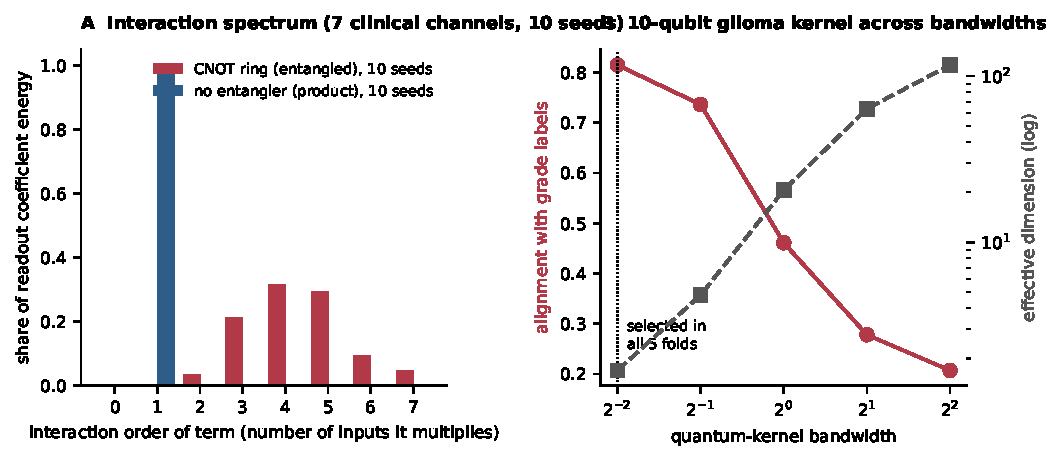
\includegraphics[width=\textwidth]{fig_v6_mechanism.pdf}
\vspace{-6pt}
\caption*{\textbf{\textsf{Figure 2 \textbar\ Mechanistic dissection of observed circuit performance and kernel geometry.}} \textbf{a}, Interaction-order coefficient energy spectrum across 10 random initialization seeds for circuits trained on the 7 clinical finding channels (Analysis C1b; red: circular CNOT ring entanglement; blue: unentangled product circuit), showing 100.0\% of non-trivial energy in interaction orders $\ge 2$ under entanglement. In the 8-qubit confirmatory architecture (incorporating the constant reference qubit $x_8 \equiv 0.0$), the effective interaction order over clinical inputs is bounded at 7. \textbf{b}, Bandwidth sweep and regularized geometric difference distance $g_\lambda(K_{\text{RBF}} \parallel K_{\text{Q}}) = 1.27 \ll \sqrt{N} = 44.72$ on 10-qubit glioma neuroimaging (M3), demonstrating classical kernel surrogacy.}
\vspace{6pt}
\end{figure*}

\begin{multicols}{2}

\section*{Discussion}

Across five reconstructible published clinical machine learning studies spanning six distinct clinical prediction tasks, none of the six published advantage claims could be verified under symmetric evaluation; where disparities existed, apparent superiority was traced to comparator undertuning, data leakage, or underpowered cohorts. In our internal chest radiograph decision-support prototype, reported calibration advantages disappeared when baselines received matched optimization and independent temperature scaling. Where empirical advantages were claimed in the audited literature, they traced to specific methodological flaws:
\begin{enumerate}
  \setlength{\itemsep}{1pt}
  \setlength{\parskip}{0pt}
  \item Calibrating only the quantum arm while leaving classical comparators uncalibrated \cite{guo2017}.
  \item Comparing tuned quantum circuits against untuned default classical implementations.
  \item Information leakage caused by fitting dimensionality reduction (PCA) prior to dataset partitioning.
  \item Partition contamination where multiple recordings or temporal epochs from the same subject crossed the train/test split.
  \item Unreproducible preprocessing pipelines and lack of code availability preventing independent verification.
\end{enumerate}

When these evaluation choices were aligned, apparent quantum utility vanished. The pre-specified confirmatory test across 56,534 held-out patients provides narrow test-sampling uncertainty: under matched default optimization (C1), the quantum circuit was materially worse on likelihood ($\Delta\text{NLL} = +0.0205$, 95\% CI 0.0186 to 0.0224), which was confirmed across 10 random initialization seeds ($\Delta\text{NLL} = +0.0142$ nats, $p = 8.43 \times 10^{-6}$; $\sigma_{\text{seed}} = 0.0045$ nats; single-checkpoint gap $+0.0205$ nats is $4.57\sigma_{\text{seed}}$), while calibration error yielded similar estimates with overlapping confidence intervals between calibrated arms. Under symmetric hyperparameter search (C2), it achieved a small likelihood advantage over linear PoE ($-0.0026$ nats) and nonlinear gated heads ($-0.0012$ nats) that fell entirely inside the pre-specified operational equivalence margin ($\pm 0.010$ nats; TOST $p < 10^{-6}$). In Analysis C2, 10-seed evaluations confirmed architectural equivalence: the mean paired difference across 10 random seeds was $\Delta\text{NLL} = -0.00067$ nats vs tuned PoE and $-0.00064$ nats vs tuned Gated Head (seed-level $p_{\text{TOST}} \le 1.50 \times 10^{-5}$), with all individual seed paired differences falling strictly within the $\pm 0.010$-nat margin. However, operational equivalence failed under class-balanced macro-averaging ($\Delta\text{NLL}_{\text{macro}} = +0.0389$ nats, $p_{\text{TOST}} > 0.99$), revealing that population-level equivalence is driven by cancellation between majority classes while the quantum circuit degrades on minority acute pathologies.

Furthermore, evaluating out-of-distribution institutional transfer from MIMIC-CXR to CheXpert revealed our largest empirical effect: the frozen quantum circuit trailed classical baselines by $\Delta\text{NLL} = \mathbf{+0.1589}$ to $\mathbf{+0.1967}$ nats (15- to 20-fold the operational equivalence margin), while all architectures experienced domain shift degradation ($\Delta\text{NLL}_{\text{shift}} = +0.120$ to $+0.143$ nats across models) due to institutional covariate shift, with empirical scale sweeps refuting periodic angle wrapping as the mechanism. When provided identical trigonometric basis features, classical order-1 Fourier regression achieved superior test likelihood (1.1123) over both tuned quantum circuits (1.1144) and classical PoE (1.1170), demonstrating that quantum expressivity in this regime is fully captured by classical models.

Importantly, our findings highlight a crucial biostatistical distinction between inconclusive comparisons on small cohorts and formal equivalence on sufficiently powered datasets \cite{altman1995}. On external benchmark tasks, wide corrected confidence intervals---such as the 95\% Nadeau--Bengio interval of approximately $-18.45$ to $+16.25$ percentage points on the heart disease low-data regime---support an \textbf{inconclusive result}, not proof that the methods are equivalent. In underpowered studies, failure to reject the null cannot establish equivalence. In contrast, in our confirmatory cohort ($N = 56,534$), the narrow 95\% confidence interval ($[-0.00359, -0.00160]$ nats) fell strictly within the operational equivalence boundary, enabling formal rejection of non-equivalence via Two One-Sided Tests ($p_{\text{TOST}} < 10^{-6}$).

For digital health, the primary implication extends beyond quantum computing. Any novel machine learning component---whether a novel neural network layer, foundation model adapter, or non-standard loss function---can appear superior under asymmetric evaluation. The 17-item checklist proposed in this work provides peer reviewers, journal editors, and healthcare technology procurement teams with an objective, code-verifiable framework to ensure that claimed improvements reflect genuine model capability rather than asymmetric care.

\subsection*{Limitations}

Our findings are subject to several boundary conditions:
\begin{enumerate}
  \setlength{\itemsep}{1pt}
  \setlength{\parskip}{0pt}
  \item \textbf{Carefully Scoped Generalizability:} Five reimplemented publications spanning six clinical prediction tasks, alongside our internal prototype, support a carefully bounded conclusion regarding shallow variational quantum circuits (5 to 11 qubits), angle encodings, and fidelity kernels on clinical tabular and imaging features. They do \textbf{not} support a universal claim that quantum machine learning can never offer an advantage in healthcare. Regimes outside our scope---including fault-tolerant quantum algorithms with asymptotic speedups, high-dimensional native quantum sensor representations, non-commuting Hamiltonian feature encodings, or molecular docking and quantum chemistry where classical simulation is fundamentally intractable---remain unaddressed by our empirical data.
  \item \textbf{Operational Statistical Nature of Equivalence Margin:} The equivalence margin of $\pm 0.010$ nats is strictly an \textbf{operational statistical benchmark} on expected negative log-likelihood differences ($\mathbb{E}[\Delta\ell] \le 0.010$ nats per prediction across the cohort), pre-specified prior to test unblinding. While it represents $\sim$0.90\% of model NLL and $\sim$3.93\% of predictive information gained over the empirical class prior, it has \textbf{not been clinically validated} against prospective patient health outcomes, diagnostic error rates, or expert clinical utility thresholds. Unless supported by prospective clinical validation studies linking margins to acceptable patient outcomes, it must remain strictly interpreted as an operational statistical benchmark. Sensitivity analysis confirms that practical equivalence holds across alternative margins from $\pm 0.020$ down to $\pm 0.005$ nats ($p_{\text{TOST}} < 10^{-4}$).
  \item \textbf{Retrospective Predictive Emulation versus Prospective Patient Outcomes:} The reported performance metrics (NLL, ECE, AUROC) evaluate retrospective mathematical emulation of an additive clinical triage rule from DenseNet finding probabilities, not direct prospective patient outcomes or real-time clinical utility. A statistically detectable difference or equivalence in retrospective log-likelihood cannot be interpreted as demonstrating clinical safety, diagnostic efficacy, or improved patient health outcomes in live hospital workflows.
  \item \textbf{Shared Early-Stopping and Calibration Partition:} Model checkpoint selection and post-hoc scalar temperature scaling were both performed separately for each model using the shared 1,600-patient development validation partition, rather than on an isolated independent calibration cohort. Reusing validation data for early stopping and temperature estimation induces a minor optimistic calibration loss bias on validation data. However, the primary confirmatory evaluation across 56,534 held-out patients remained strictly unblended and untouched during all training and calibration stages, guaranteeing that reported test-set generalization metrics are completely leak-free.
  \item \textbf{Noise Ceiling of Clinical Targets:} The clinical target in our chest radiograph system is derived from report labeler heuristics and clinical decision-support rules rather than adjudicated clinician consensus, while the inputs are noisy DenseNet probability estimates. Non-differential label extraction noise and upstream perceptual ambiguity bound the accuracy ceiling at $\approx 54.4\%$. Equivalence near this noise floor demonstrates that shallow quantum circuits do not overcome representation noise, rather than demonstrating equivalence across noiseless tasks.
  \item \textbf{Single-Center Institution Effects:} While the 56,534-patient cohort ensures patient independence and eliminates intra-subject clustering, it represents a single medical institution (Stanford Hospital); multi-center transfer from MIMIC-CXR to CheXpert demonstrated performance degradation under domain shift ($\Delta\text{NLL} = +0.1589$ nats vs PoE, $+0.1967$ vs Logistic Regression).
  \item \textbf{Hardware and Simulation Boundary:} Empirical quantum evaluations were conducted at 5 to 11 qubits under exact classical statevector simulation. Prior physical noise simulations indicate that physical hardware decoherence further widens the classical advantage.
  \item \textbf{Literature Selection and Reconstructibility:} The literature audit was restricted to studies with open data and reconstructible pipelines; three studies were non-reconstructible due to unreleased code or proprietary features. In the case of chronic kidney disease (Parthasarathi et al.), the published 99.2\% accuracy claim utilized an under-specified sparse autoencoder and Kalman filter that could not be verified from the paper text, representing an important documentation barrier.
  \item \textbf{Single-Rater Checklist Scoring:} The 17-item checklist was scored by a single rater (S.R.M.), though operationalized via objective binary criteria without manufactured second-reviewer ratings.
\end{enumerate}

\section*{Methods}

\subsection*{Algorithm: Symmetric Evaluation Protocol}

To ensure complete reproducibility and eliminate evaluation asymmetries, all comparative analyses adhered to the formal procedure specified in \textbf{Algorithm 1}.

\begin{lstlisting}[language=Python, mathescape=true, caption={Algorithm 1: Symmetric Evaluation Protocol for Clinical Prediction Models.}]
Algorithm 1: Symmetric Evaluation Protocol
Input: Dataset $\mathcal{D} = \{(x_i, y_i, g_i)\}$ with patient identifiers $g_i$;
       Quantum family $\mathcal{M}_{\text{Q}}$ with search grid $\Theta_{\text{Q}}$;
       Classical families $\mathcal{M}_{\text{C}}$ with search grid $\Theta_{\text{C}}$;
       Operational margin $\Delta_{\text{equiv}} = \pm 0.010$ nats; significance $\alpha = 0.05$.
Output: Paired shifts $\bar{d}$, dependency-corrected 95% CIs, p-values, decision verdict.

1. Partitioning at Unit of Independence (Rule P3):
   Partition $\mathcal{D}$ into $J \times K$ outer folds grouped strictly by patient ID $g_i$
   such that no patient crosses fold boundaries ($S_{\text{train}} \cap S_{\text{test}} = \emptyset$).
2. Leak-Free In-Fold Preprocessing (Rule P3):
   For each outer fold $(j, k)$:
     Fit imputer, standardizer, and PCA strictly on $\mathcal{D}_{\text{train}}^{(j, k)}$.
     Apply fitted transformers to $\mathcal{D}_{\text{train}}^{(j, k)}$ and $\mathcal{D}_{\text{test}}^{(j, k)}$.
3. Matched Hyperparameter Tuning (Rule P2):
   Within $\mathcal{D}_{\text{train}}^{(j, k)}$, run 3-fold inner cross-validation:
     $\theta_{\text{Q}}^* = \arg\min \text{NLL}_{\text{inner}}(\theta)$ over $\Theta_{\text{Q}}$.
     $\theta_{\text{C}}^* = \arg\min \text{NLL}_{\text{inner}}(\theta)$ over $\Theta_{\text{C}}$.
4. Model Selection and Calibration (Rules P1, P2):
   Retain frozen checkpoint $\theta^*$ trained on $\mathcal{D}_{\text{train}}^{(j, k)}$ at validation minimum (no refit).
   Fit scalar temperature parameter $T^*$ separately per model on development validation logits:
     $T^* = \arg\min \text{NLL}(y_{\text{val}}, \text{softmax}(z / T))$.
   (Note: Performing calibration separately per model using the shared development validation
   partition induces minor optimistic validation loss bias; test data $\mathcal{D}_{\text{test}}^{(j, k)}$ remain strictly sealed.)
5. Held-Out Evaluation (Rules P5, P6):
   Score frozen, calibrated models on untouched held-out $\mathcal{D}_{\text{test}}^{(j, k)}$:
     Compute paired difference $d_{(j, k)} = \text{Metric}_{\text{Q}}^{(j, k)} - \text{Metric}_{\text{C}}^{(j, k)}$.
6. Inferential Analysis (Rule P4):
   If repeated cross-validation ($J \times K$ outer folds):
     Calculate Nadeau-Bengio corrected variance: $\sigma_{\text{NB}}^2 = \left(\frac{1}{JK} + \frac{n_{\text{test}}}{n_{\text{train}}}\right) S^2$.
     Compute test statistic $t_{\text{NB}} = \bar{d} / \sigma_{\text{NB}}$ with $\nu = JK - 1$ degrees of freedom.
   If confirmatory cohort ($N$ paired patients) or multi-seed evaluation ($S$ seeds):
     Conduct Schuirmann Two One-Sided Tests (TOST) against $[-\Delta_{\text{equiv}}, +\Delta_{\text{equiv}}]$:
       $t_1 = (\bar{d} + \Delta_{\text{equiv}}) / \text{SE}$;  $p_1 = 1 - F_t(t_1; \nu)$
       $t_2 = (\bar{d} - \Delta_{\text{equiv}}) / \text{SE}$;  $p_2 = F_t(t_2; \nu)$
       $p_{\text{TOST}} = \max(p_1, p_2)$.
7. Decision Verdict:
   Assign: Not Reproduced, Inconclusive, Collapsed to Chance, or Practically Equivalent.
\end{lstlisting}

\subsection*{Cohort Construction, Deduplication, and Independence Architecture}
\begin{itemize}
  \setlength{\itemsep}{1pt}
  \item \textbf{MIMIC-CXR-JPG (v2.0.0):} Evaluated under PhysioNet Credentialed Health Data License 1.5.0 \cite{johnson2019}. Restricted to one frontal study per patient (highest study index), partitioned into 1,338 training, 446 calibration, and 447 test studies.
  \item \textbf{CheXpert-v1.0-Small Cohort Construction:} Used under Stanford Research Data Agreement \cite{irvin2019}. To guarantee patient independence and prevent intra-cluster correlation from repeated longitudinal visits, the cohort was filtered strictly to frontal examinations (AP/PA), and exactly one study per unique human subject was selected deterministically by taking the final encounter (highest study ID). The initial 8,000 unique patients were partitioned into 6,400 training and 1,600 calibration studies for development. All 56,534 subsequent unique frontal studies formed the untouched confirmatory test set. Patient-level set intersection confirmed 0 patient overlap ($|S_{\text{dev}} \cap S_{\text{test}}| = 0$). Unit tests (\texttt{test\_one\_study\_per\_patient.py}) enforce that repeated subject rows are excluded before dataset assembly.
  \item \textbf{BraTS 2020:} 369 official glioma subjects (293 HGG, 76 LGG) \cite{bakas2017}. Feature extraction embeddings were derived using the served foundation checkpoint, with 111 subjects strictly held out from encoder training.
  \item \textbf{Literature Benchmark Cohorts:} UCI Chronic Kidney Disease ($n=400$), UCI Parkinson's Disease Voice ($n=195$, 31 subjects), UCI Pima Indian Diabetes ($n=768$), MSU Adolescent Schizophrenia EEG ($n=84$), UCI Heart Disease ($n=918$), and TCGA Glioma ($n=839$).
\end{itemize}

\subsection*{Variational Circuit Architecture and Parameter Counts}
The input feature vector $x \in [0, 1]^8$ consists of seven normalized radiological finding probabilities extracted via DenseNet-121 ($x_1, \dots, x_7$) and a constant baseline reference channel $x_8 \equiv 0.0$. Features are mapped via single-qubit angle rotations $R_Y(\pi s x_i)|0\rangle$. Because $x_8 \equiv 0$, the eighth qubit receives a zero rotation angle $R_Y(0)|0\rangle = |0\rangle$ and remains initialized in the unrotated ground state, providing an unrotated reference baseline coupled to qubits 7 and 1 through the closed CNOT entangling ring. Expectation values of Pauli-$Z$ observables $\langle Z_k \rangle(x) \in [-1, 1]$ across all 8 qubits are projected to 6 class logits via linear readout $W_{\text{out}} \langle Z \rangle(x) + b_{\text{out}}$ (corresponding to the six triage categories: Normal, Pneumonia, Heart Failure, COPD, Malignancy, Pneumothorax). In CheXpert, because automated report labeling lacks the \texttt{hyperinflation} finding, Acuity Class 3 (COPD) has zero positive occurrences in both development and confirmatory test partitions ($y \in \{0, 1, 2, 4, 5\}$). Forward inference and calibration symmetrically compute full 6-way softmax probabilities across all models; sample NLL is evaluated as $-\ln \hat{p}_{i, y_i}$ for observed ground-truth labels $y_i$, while multi-class AUROC is macro-averaged across the 5 observed positive classes to prevent zero-denominator division. Parameter counts are: default C1 VQC ($L=3$, 48 angles $+ 54$ readout weights = \textbf{102 parameters}); optimal C2 VQC ($L=4$, 64 angles $+ 54$ readout weights = \textbf{118 parameters}); linear Product-of-Experts ($6 \times 8 + 6 = \mathbf{54\text{ parameters}}$); Logistic Regression ($6 \times 8 + 6 = \mathbf{54\text{ parameters}}$); and nonlinear Gated Head (64 gating weights $+ 8$ gating biases $+ 54$ readout parameters = \textbf{126 parameters}). During development, the 1,600 calibration patients were used for early-stopping checkpoint selection and scalar temperature scaling \cite{guo2017} without pooled refitting. Calibration was performed separately for each model arm using this shared development validation partition (not on an independent external calibration cohort). The 56,534 test patients were strictly held out and scored without any selection or temperature refitting on them.

\subsection*{Circuit Simulation and Mathematical Verification}
Quantum circuits were evaluated using an optimized PyTorch batched statevector engine. Prior to evaluation, the simulator was verified against PennyLane (\texttt{default.qubit}) on 1,000 random input/parameter pairs at 7 and 8 qubits for both entangled and unentangled topologies; maximum absolute discrepancy was $7.77 \times 10^{-16}$, confirming numerical equivalence to double-precision machine tolerance.

\subsection*{Statistical Inference and Equivalence Margins}
Model calibration and discrimination are evaluated via Negative Log-Likelihood (NLL) and Expected Calibration Error (ECE):
\begin{equation}
\text{NLL}(y, \hat{p}) = -\frac{1}{N} \sum_{i=1}^N \sum_{c=1}^C y_{ic} \ln \hat{p}_{ic}
\end{equation}
\begin{equation}
\text{ECE} = \sum_{m=1}^M \frac{|B_m|}{N} |\text{acc}(B_m) - \text{conf}(B_m)|
\end{equation}
Under our metric directionality, the paired likelihood difference is defined as:
\begin{equation}
\Delta\text{NLL} = \text{NLL}_{\text{quantum}} - \text{NLL}_{\text{classical}}
\end{equation}
where $\Delta\text{NLL} > 0$ indicates classical superiority (lower loss) and $\Delta\text{NLL} < 0$ indicates quantum superiority.

To test practical statistical equivalence on the confirmatory cohort, Two One-Sided Tests (TOST) \cite{schuirmann1987,lakens2017} evaluate the composite null hypothesis $H_0: \mu_d \le -\Delta_{\text{equiv}} \text{ or } \mu_d \ge +\Delta_{\text{equiv}}$ against the alternative $H_1: -\Delta_{\text{equiv}} < \mu_d < +\Delta_{\text{equiv}}$ under the operational margin $\Delta_{\text{equiv}} = \pm 0.010$ nats:
\begin{equation}
t_1 = \frac{\bar{d} - (-\Delta_{\text{equiv}})}{\text{SE}(\bar{d})}, \quad t_2 = \frac{\bar{d} - (+\Delta_{\text{equiv}})}{\text{SE}(\bar{d})}
\end{equation}
\begin{equation}
p_1 = 1 - F_t(t_1; \nu), \quad p_2 = F_t(t_2; \nu), \quad p_{\text{TOST}} = \max(p_1, p_2)
\end{equation}
where $F_t(\cdot; \nu)$ denotes the cumulative distribution function of Student's $t$-distribution with $\nu$ degrees of freedom (equivalently written with $t_2' = \frac{+\Delta_{\text{equiv}} - \bar{d}}{\text{SE}(\bar{d})}$ and $p_2 = 1 - F_t(t_2'; \nu)$). For the massive confirmatory cohort ($N = 56,534$, $\nu = 56,533$), $F_t$ converges asymptotically to the standard normal CDF $\Phi$; for the 10-seed initialization analysis ($\nu = 9$), Student's $t$-distribution with 9 degrees of freedom is strictly evaluated. Equivalence at significance $\alpha = 0.05$ is established when $p_{\text{TOST}} < 0.05$, which is mathematically equivalent to the 90\% confidence interval falling strictly inside $[-\Delta_{\text{equiv}}, +\Delta_{\text{equiv}}]$.

\begin{itemize}
  \setlength{\itemsep}{1pt}
  \item \textbf{Likelihood Contrasts:} Wilcoxon signed-rank tests for paired median shifts, paired Student's $t$-intervals for mean differences, and Two One-Sided Tests (TOST) with a prespecified operational average-NLL statistical equivalence margin of $\Delta_{\text{equiv}} = \pm 0.010$ nats.
  \item \textbf{Classification Accuracy:} McNemar's exact test for paired binary proportions.
  \item \textbf{Discrimination:} DeLong's test for correlated ROC curves \cite{delong1988}.
  \item \textbf{Multiple Testing:} Holm--Bonferroni correction applied across the family of pairwise contrasts.
  \item \textbf{Resampling:} 10,000 patient-clustered bootstrap resamples for parameter difference confidence intervals.
  \item \textbf{Cross-Validation Corrected Inference:} Nadeau--Bengio corrected resampled $t$-test for 5 $\times$ 5 repeated cross-validation \cite{nadeau2003}:
  \begin{equation}
  \hat{\sigma}^2_{\text{corrected}} = \left(\frac{1}{JK} + \frac{n_{\text{test}}}{n_{\text{train}}}\right) S^2
  \end{equation}
  preventing false-positive inflation from fold overlap.
\end{itemize}

\section*{Ethics Statement}
This study represents a secondary computational analysis of preexisting, publicly accessible and credentialed, fully de-identified biomedical datasets: CheXpert \cite{irvin2019}, MIMIC-CXR-JPG \cite{johnson2019}, BraTS 2020 \cite{bakas2017}, and open machine learning benchmarks. The original clinical data collection, participant consent protocols, and database creation were approved by the respective institutional review boards (IRBs) of the originating institutions: the Stanford University Institutional Review Board for CheXpert, and the Institutional Review Boards of Beth Israel Deaconess Medical Center and the Massachusetts Institute of Technology for MIMIC-CXR, with waivers of informed consent granted by those bodies for the release of retrospective de-identified records under Health Insurance Portability and Accountability Act (HIPAA) Safe Harbor provisions. Access to MIMIC-CXR-JPG was granted to the author under PhysioNet Credentialed Health Data Use License 1.5.0 following completion of required human research ethics training. Access to CheXpert was governed by the Stanford AIMI Research Data Use Agreement. Access to BraTS 2020 was governed by The Cancer Imaging Archive (TCIA) Data Usage Policy. Because this work involved exclusively secondary computational analysis of preexisting, fully de-identified records without direct patient interaction, clinical intervention, or access to identifiable private health information, separate institutional review was not required for this secondary analysis under applicable data-use and institutional policies. No prospective clinical trial registration was required.

\section*{Data Availability}
MIMIC-CXR-JPG and CheXpert datasets are available to credentialed researchers via PhysioNet (\url{physionet.org}) and Stanford University (\url{aimi.stanford.edu}). BraTS 2020 is available via the Synapse repository. All derived aggregate metrics, parameter checkpoints, and prediction arrays are available in the project repository.

\section*{Code Availability}
All experimental code, simulation harnesses, audit pipelines, and verification tests are openly available at: \url{https://github.com/Sivaguru-2008/aura}. The Level A data provenance and numerical drift verification suite (recomputing all primary metrics and figures from saved model checkpoints in $\sim$19 seconds) can be executed via: \texttt{python reproduce\_paper.py}. Level B re-scoring of TOST statistics and bootstrap intervals from prediction tensors takes $\sim$5 minutes. Full Level C end-to-end retraining instructions across all 36 configurations and feature extraction pipelines ($\sim$16 hours compute) are detailed in Supplementary Note 7.

\section*{Acknowledgements}
The author thanks the PhysioNet, Stanford AIMI, TCGA, BraTS, and UCI Machine Learning repository teams for curating and hosting the open-access and credentialed clinical datasets.

\section*{Author Contributions}
S.R.M. conceived the study, developed the symmetric evaluation protocol, designed and implemented the quantum simulation and classical comparison frameworks, re-implemented the published literature studies, performed the pre-specified confirmatory statistical analyses, and wrote the manuscript.

\section*{Competing Interests}
The author declares no competing financial or non-financial interests.

\small
\begin{thebibliography}{99}
\setlength{\itemsep}{1pt}
\setlength{\parskip}{0pt}
\bibitem{gupta2025} Gupta, S. et al. Quantum machine learning in digital health: a systematic review. \textit{npj Digit. Med.} \textbf{8}, 42 (2025).
\bibitem{rendle2019} Rendle, S. et al. Are we really making much progress? A worrying analysis of recent neural recommendation approaches. In \textit{Proc. RecSys} 101--109 (2019).
\bibitem{musgrave2020} Musgrave, K. et al. A metric learning reality check. In \textit{Proc. ECCV} 681--699 (2020).
\bibitem{henderson2018} Henderson, P. et al. Deep reinforcement learning that matters. In \textit{Proc. AAAI} 3207--3214 (2018).
\bibitem{glocker2022} Glocker, B. et al. Machine learning for medical image analysis: are we making progress? \textit{Lancet Digit. Health} \textbf{4}, e680--e681 (2022).
\bibitem{kochkov2021} Kochkov, D. et al. Machine learning-accelerated computational fluid dynamics. \textit{Proc. Natl. Acad. Sci. USA} \textbf{118}, e2101784118 (2021).
\bibitem{kubler2021} K{\"u}bler, J. et al. The inductive bias of quantum kernels. In \textit{Proc. NeurIPS} 12661--12673 (2021).
\bibitem{biamonte2017} Biamonte, J. et al. Quantum machine learning. \textit{Nature} \textbf{549}, 195--202 (2017).
\bibitem{cerezo2021} Cerezo, M. et al. Variational quantum algorithms. \textit{Nat. Rev. Phys.} \textbf{3}, 625--644 (2021).
\bibitem{huang2021power} Huang, H.-Y. et al. Power of data in quantum machine learning. \textit{Nat. Commun.} \textbf{12}, 2631 (2021).
\bibitem{thanasilp2023} Thanasilp, S. et al. Exponential concentration and untrainability in quantum kernel methods. \textit{Quantum} \textbf{7}, 1153 (2023).
\bibitem{shaydulin2022} Shaydulin, R. et al. Importance of kernel bandwidth in quantum machine learning. \textit{Phys. Rev. A} \textbf{106}, 042407 (2022).
\bibitem{mcclean2018} McClean, J. R. et al. Barren plateaus in quantum neural network training landscapes. \textit{Nat. Commun.} \textbf{9}, 4812 (2018).
\bibitem{nadeau2003} Nadeau, C. \& Bengio, Y. Inference for the generalization error. \textit{Mach. Learn.} \textbf{52}, 239--281 (2003).
\bibitem{parthasarathi2025} Parthasarathi, P. et al. Variational quantum classifier-based early identification and classification of chronic kidney disease using sparse autoencoder and LASSO shrinkage. \textit{PeerJ Comput. Sci.} \textbf{11}, e2789 (2025).
\bibitem{daga2026} Daga, M., Naole, S. et al. Adaptive quantum kernel selection via leakage-free stacking for clinical diagnostics on NISQ hardware. \textit{Sci. Rep.} \textbf{16}, 12841 (2026).
\bibitem{aksoy2024} Aksoy, G. \& Cattan, G. Quantum machine-based decision support system for the detection of schizophrenia from EEG records. \textit{J. Med. Syst.} \textbf{48}, 29 (2024).
\bibitem{akpinar2025} Akpinar, E. \& Oduncuoglu, M. Hybrid classical and quantum computing for enhanced glioma tumor classification using TCGA data. \textit{Sci. Rep.} \textbf{15}, 25935 (2025).
\bibitem{ghisoni2026} Ghisoni, F., Borrotti, M. \& Mariani, P. A large scale statistical analysis of quantum and classical neural networks in the medical domain. \textit{Sci. Rep.} \textbf{16}, 3719 (2026).
\bibitem{jahin2025} Jahin, M. A. et al. KACQ-DCNN: Uncertainty-aware interpretable Kolmogorov-Arnold classical-quantum dual-channel neural network for heart disease detection. \textit{Comput. Biol. Med.} \textbf{197}, 110976 (2025).
\bibitem{chen2026} Chen, P. et al. Prostate cancer classification using quantum machine learning on multi-parametric MRI. \textit{Proc. SPIE} \textbf{13930}, 139300K (2026).
\bibitem{choi2026} Choi, J. et al. Performance evaluation of quantum support vector machine for COVID-19 biomarker analysis. \textit{Comput. Methods Programs Biomed.} \textbf{281}, 109343 (2026).
\bibitem{johnson2019} Johnson, A. E. W. et al. MIMIC-CXR-JPG, a large publicly available database of labeled chest radiographs. \textit{Sci. Data} \textbf{6}, 317 (2019).
\bibitem{irvin2019} Irvin, J. et al. CheXpert: A large chest radiograph dataset with uncertainty labels and expert comparison. In \textit{Proc. AAAI} 590--597 (2019).
\bibitem{bakas2017} Bakas, S. et al. Advancing the cancer genome atlas glioma analysis with multimodal brain tumor segmentation (BraTS). \textit{Sci. Data} \textbf{4}, 170188 (2017).
\bibitem{collins2021} Collins, G. S. et al. Protocol for development of TRIPOD+AI: a reporting guideline for diagnostic and prognostic prediction models based on artificial intelligence. \textit{BMJ Open} \textbf{11}, e048008 (2021).
\bibitem{schuld2021effect} Schuld, M., Sweke, R. \& Meyer, J. J. Effect of data encoding on the expressive power of variational quantum-machine-learning models. \textit{Phys. Rev. A} \textbf{103}, 032430 (2021).
\bibitem{geirhos2020} Geirhos, R. et al. Shortcut learning in deep neural networks. \textit{Nat. Mach. Intell.} \textbf{2}, 665--673 (2020).
\bibitem{liu2020consort} Liu, X. et al. Reporting guidelines for clinical trial reports for interventions involving artificial intelligence: the CONSORT-AI extension. \textit{Nat. Med.} \textbf{26}, 1364--1374 (2020).
\bibitem{platt1999} Platt, J. C. Probabilistic outputs for support vector machines and comparisons to regularized likelihood methods. \textit{Adv. Large Margin Classif.} \textbf{10}, 61--74 (1999).
\bibitem{guo2017} Guo, C., Pleiss, G., Sun, Y. \& Weinberger, K. Q. On calibration of modern neural networks. In \textit{Proc. ICML} 1321--1330 (2017).
\bibitem{schuirmann1987} Schuirmann, D. J. A comparison of the two one-sided tests procedure and the power approach for assessing the equivalence of average bioavailability. \textit{J. Pharmacokinet. Biopharm.} \textbf{15}, 657--680 (1987).
\bibitem{lakens2017} Lakens, D. Equivalence testing for psychological research: a tutorial on TOST design, power, and statistical analyses. \textit{Soc. Psychol. Personal. Sci.} \textbf{8}, 355--362 (2017).
\bibitem{delong1988} DeLong, E. R., DeLong, D. M. \& Clarke-Pearson, D. Learning to compare the areas under two or more correlated receiver operating characteristic curves: a nonparametric approach. \textit{Biometrics} \textbf{44}, 837--845 (1988).
% uncited reference jaeschke1994 removed
\bibitem{altman1995} Altman, D. G. \& Bland, J. M. Absence of evidence is not evidence of absence. \textit{BMJ} \textbf{311}, 485 (1995).
\end{thebibliography}

\end{multicols}

\end{document}
